\documentclass[1p]{elsarticle_modified}
%\bibliographystyle{elsarticle-num}

%\usepackage[colorlinks]{hyperref}
%\usepackage{abbrmath_seonhwa} %\Abb, \Ascr, \Acal ,\Abf, \Afrak
\usepackage{amsfonts}
\usepackage{amssymb}
\usepackage{amsmath}
\usepackage{amsthm}
\usepackage{scalefnt}
\usepackage{amsbsy}
\usepackage{kotex}
\usepackage{caption}
\usepackage{subfig}
\usepackage{color}
\usepackage{graphicx}
\usepackage{xcolor} %% white, black, red, green, blue, cyan, magenta, yellow
\usepackage{float}
\usepackage{setspace}
\usepackage{hyperref}

\usepackage{tikz}
\usetikzlibrary{arrows}

\usepackage{multirow}
\usepackage{array} % fixed length table
\usepackage{hhline}

%%%%%%%%%%%%%%%%%%%%%
\makeatletter
\renewcommand*\env@matrix[1][\arraystretch]{%
	\edef\arraystretch{#1}%
	\hskip -\arraycolsep
	\let\@ifnextchar\new@ifnextchar
	\array{*\c@MaxMatrixCols c}}
\makeatother %https://tex.stackexchange.com/questions/14071/how-can-i-increase-the-line-spacing-in-a-matrix
%%%%%%%%%%%%%%%

\usepackage[normalem]{ulem}

\newcommand{\msout}[1]{\ifmmode\text{\sout{\ensuremath{#1}}}\else\sout{#1}\fi}
%SOURCE: \msout is \stkout macro in https://tex.stackexchange.com/questions/20609/strikeout-in-math-mode

\newcommand{\cancel}[1]{
	\ifmmode
	{\color{red}\msout{#1}}
	\else
	{\color{red}\sout{#1}}
	\fi
}

\newcommand{\add}[1]{
	{\color{blue}\uwave{#1}}
}

\newcommand{\replace}[2]{
	\ifmmode
	{\color{red}\msout{#1}}{\color{blue}\uwave{#2}}
	\else
	{\color{red}\sout{#1}}{\color{blue}\uwave{#2}}
	\fi
}

\newcommand{\Sol}{\mathcal{S}} %segment
\newcommand{\D}{D} %diagram
\newcommand{\A}{\mathcal{A}} %arc


%%%%%%%%%%%%%%%%%%%%%%%%%%%%%5 test

\def\sl{\operatorname{\textup{SL}}(2,\Cbb)}
\def\psl{\operatorname{\textup{PSL}}(2,\Cbb)}
\def\quan{\mkern 1mu \triangleright \mkern 1mu}

\theoremstyle{definition}
\newtheorem{thm}{Theorem}[section]
\newtheorem{prop}[thm]{Proposition}
\newtheorem{lem}[thm]{Lemma}
\newtheorem{ques}[thm]{Question}
\newtheorem{cor}[thm]{Corollary}
\newtheorem{defn}[thm]{Definition}
\newtheorem{exam}[thm]{Example}
\newtheorem{rmk}[thm]{Remark}
\newtheorem{alg}[thm]{Algorithm}

\newcommand{\I}{\sqrt{-1}}
\begin{document}

%\begin{frontmatter}
%
%\title{Boundary parabolic representations of knots up to 8 crossings}
%
%%% Group authors per affiliation:
%\author{Yunhi Cho} 
%\address{Department of Mathematics, University of Seoul, Seoul, Korea}
%\ead{yhcho@uos.ac.kr}
%
%
%\author{Seonhwa Kim} %\fnref{s_kim}}
%\address{Center for Geometry and Physics, Institute for Basic Science, Pohang, 37673, Korea}
%\ead{ryeona17@ibs.re.kr}
%
%\author{Hyuk Kim}
%\address{Department of Mathematical Sciences, Seoul National University, Seoul 08826, Korea}
%\ead{hyukkim@snu.ac.kr}
%
%\author{Seokbeom Yoon}
%\address{Department of Mathematical Sciences, Seoul National University, Seoul, 08826,  Korea}
%\ead{sbyoon15@snu.ac.kr}
%
%\begin{abstract}
%We find all boundary parabolic representation of knots up to 8 crossings.
%
%\end{abstract}
%\begin{keyword}
%    \MSC[2010] 57M25 
%\end{keyword}
%
%\end{frontmatter}

%\linenumbers
%\tableofcontents
%
\newcommand\colored[1]{\textcolor{white}{\rule[-0.35ex]{0.8em}{1.4ex}}\kern-0.8em\color{red} #1}%
%\newcommand\colored[1]{\textcolor{white}{ #1}\kern-2.17ex	\textcolor{white}{ #1}\kern-1.81ex	\textcolor{white}{ #1}\kern-2.15ex\color{red}#1	}

{\Large $\underline{12a_{0352}~(K12a_{0352})}$}

\setlength{\tabcolsep}{10pt}
\renewcommand{\arraystretch}{1.6}
\vspace{1cm}\begin{tabular}{m{100pt}>{\centering\arraybackslash}m{274pt}}
\multirow{5}{120pt}{
	\centering
	\includegraphics[width=112pt]{../../../GIT/diagram.site/Diagrams/png/1153_12a_0352.png}\\
\ \ \ A knot diagram\footnotemark}&
\allowdisplaybreaks
\textbf{Linearized knot diagam} \\
\cline{2-2}
 &
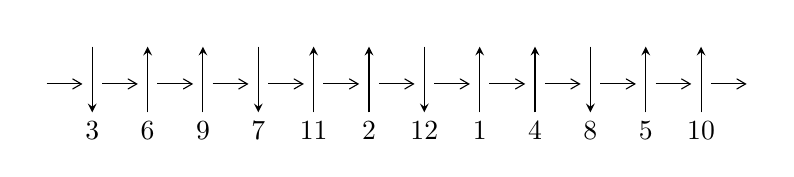
\begin{tikzpicture}[x=20pt, y=17pt]
	% nodes
	\node (C0) at (0, 0) {};
	\node (C1) at (1, 0) {};
	\node (C1U) at (1, +1) {};
	\node (C1D) at (1, -1) {3};

	\node (C2) at (2, 0) {};
	\node (C2U) at (2, +1) {};
	\node (C2D) at (2, -1) {6};

	\node (C3) at (3, 0) {};
	\node (C3U) at (3, +1) {};
	\node (C3D) at (3, -1) {9};

	\node (C4) at (4, 0) {};
	\node (C4U) at (4, +1) {};
	\node (C4D) at (4, -1) {7};

	\node (C5) at (5, 0) {};
	\node (C5U) at (5, +1) {};
	\node (C5D) at (5, -1) {11};

	\node (C6) at (6, 0) {};
	\node (C6U) at (6, +1) {};
	\node (C6D) at (6, -1) {2};

	\node (C7) at (7, 0) {};
	\node (C7U) at (7, +1) {};
	\node (C7D) at (7, -1) {12};

	\node (C8) at (8, 0) {};
	\node (C8U) at (8, +1) {};
	\node (C8D) at (8, -1) {1};

	\node (C9) at (9, 0) {};
	\node (C9U) at (9, +1) {};
	\node (C9D) at (9, -1) {4};

	\node (C10) at (10, 0) {};
	\node (C10U) at (10, +1) {};
	\node (C10D) at (10, -1) {8};

	\node (C11) at (11, 0) {};
	\node (C11U) at (11, +1) {};
	\node (C11D) at (11, -1) {5};

	\node (C12) at (12, 0) {};
	\node (C12U) at (12, +1) {};
	\node (C12D) at (12, -1) {10};
	\node (C13) at (13, 0) {};

	% arrows
	\draw[->,>={angle 60}]
	(C0) edge (C1) (C1) edge (C2) (C2) edge (C3) (C3) edge (C4) (C4) edge (C5) (C5) edge (C6) (C6) edge (C7) (C7) edge (C8) (C8) edge (C9) (C9) edge (C10) (C10) edge (C11) (C11) edge (C12) (C12) edge (C13) ;	\draw[->,>=stealth]
	(C1U) edge (C1D) (C2D) edge (C2U) (C3D) edge (C3U) (C4U) edge (C4D) (C5D) edge (C5U) (C6D) edge (C6U) (C7U) edge (C7D) (C8D) edge (C8U) (C9D) edge (C9U) (C10U) edge (C10D) (C11D) edge (C11U) (C12D) edge (C12U) ;
	\end{tikzpicture} \\
\hhline{~~} \\& 
\textbf{Solving Sequence} \\ \cline{2-2} 
 &
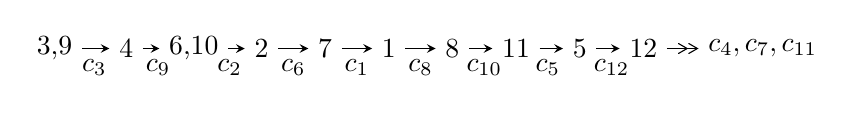
\begin{tikzpicture}[x=23pt, y=7pt]
	% node
	\node (A0) at (-1/8, 0) {3,9};
	\node (A1) at (1, 0) {4};
	\node (A2) at (33/16, 0) {6,10};
	\node (A3) at (25/8, 0) {2};
	\node (A4) at (33/8, 0) {7};
	\node (A5) at (41/8, 0) {1};
	\node (A6) at (49/8, 0) {8};
	\node (A7) at (57/8, 0) {11};
	\node (A8) at (65/8, 0) {5};
	\node (A9) at (73/8, 0) {12};
	\node (C1) at (1/2, -1) {$c_{3}$};
	\node (C2) at (3/2, -1) {$c_{9}$};
	\node (C3) at (21/8, -1) {$c_{2}$};
	\node (C4) at (29/8, -1) {$c_{6}$};
	\node (C5) at (37/8, -1) {$c_{1}$};
	\node (C6) at (45/8, -1) {$c_{8}$};
	\node (C7) at (53/8, -1) {$c_{10}$};
	\node (C8) at (61/8, -1) {$c_{5}$};
	\node (C9) at (69/8, -1) {$c_{12}$};
	\node (A10) at (11, 0) {$c_{4},c_{7},c_{11}$};

	% edge
	\draw[->,>=stealth]	
	(A0) edge (A1) (A1) edge (A2) (A2) edge (A3) (A3) edge (A4) (A4) edge (A5) (A5) edge (A6) (A6) edge (A7) (A7) edge (A8) (A8) edge (A9) ;
	\draw[->>,>={angle 60}]	
	(A9) edge (A10);
\end{tikzpicture} \\ 

\end{tabular} \\

\footnotetext{
The image of knot diagram is generated by the software ``\textbf{Draw programme}" developed by Andrew Bartholomew(\url{http://www.layer8.co.uk/maths/draw/index.htm\#Running-draw}), where we modified some parts for our purpose(\url{https://github.com/CATsTAILs/LinksPainter}).
}\phantom \\ \newline 
\centering \textbf{Ideals for irreducible components\footnotemark of $X_{\text{par}}$} 
 
\begin{align*}
I^u_{1}&=\langle 
2.96609\times10^{1105} u^{176}-3.83738\times10^{1104} u^{175}+\cdots+6.11633\times10^{1104} b-9.51664\times10^{1107},\\
\phantom{I^u_{1}}&\phantom{= \langle  }-2.51616\times10^{1108} u^{176}+1.20236\times10^{1107} u^{175}+\cdots+1.95111\times10^{1107} a+7.44748\times10^{1110},\\
\phantom{I^u_{1}}&\phantom{= \langle  }u^{177}- u^{176}+\cdots+24611 u+319\rangle \\
I^u_{2}&=\langle 
1.02869\times10^{49} u^{47}-3.44127\times10^{48} u^{46}+\cdots+1.10032\times10^{48} b+1.08498\times10^{49},\\
\phantom{I^u_{2}}&\phantom{= \langle  }-1.92965\times10^{50} u^{47}-2.46970\times10^{50} u^{46}+\cdots+1.44141\times10^{50} a+3.77821\times10^{50},\\
\phantom{I^u_{2}}&\phantom{= \langle  }u^{48}-15 u^{46}+\cdots-12 u^2+1\rangle \\
\\
\end{align*}
\raggedright * 2 irreducible components of $\dim_{\mathbb{C}}=0$, with total 225 representations.\\
\footnotetext{All coefficients of polynomials are rational numbers. But the coefficients are sometimes approximated in decimal forms when there is not enough margin.}
\newpage
\renewcommand{\arraystretch}{1}
\centering \section*{I. $I^u_{1}= \langle 2.97\times10^{1105} u^{176}-3.84\times10^{1104} u^{175}+\cdots+6.12\times10^{1104} b-9.52\times10^{1107},\;-2.52\times10^{1108} u^{176}+1.20\times10^{1107} u^{175}+\cdots+1.95\times10^{1107} a+7.45\times10^{1110},\;u^{177}- u^{176}+\cdots+24611 u+319 \rangle$}
\flushleft \textbf{(i) Arc colorings}\\
\begin{tabular}{m{7pt} m{180pt} m{7pt} m{180pt} }
\flushright $a_{3}=$&$\begin{pmatrix}1\\0\end{pmatrix}$ \\
\flushright $a_{9}=$&$\begin{pmatrix}0\\u\end{pmatrix}$ \\
\flushright $a_{4}=$&$\begin{pmatrix}1\\- u^2\end{pmatrix}$ \\
\flushright $a_{6}=$&$\begin{pmatrix}12.8960 u^{176}-0.616241 u^{175}+\cdots-303378. u-3817.04\\-4.84946 u^{176}+0.627398 u^{175}+\cdots+121459. u+1555.94\end{pmatrix}$ \\
\flushright $a_{10}=$&$\begin{pmatrix}u\\- u^3+u\end{pmatrix}$ \\
\flushright $a_{2}=$&$\begin{pmatrix}-1.21098 u^{176}-2.03163 u^{175}+\cdots+18885.2 u+182.856\\7.95313 u^{176}+0.537132 u^{175}+\cdots-197423. u-2528.22\end{pmatrix}$ \\
\flushright $a_{7}=$&$\begin{pmatrix}-12.9583 u^{176}+1.34468 u^{175}+\cdots+396686. u+5007.98\\13.5311 u^{176}-1.03585 u^{175}+\cdots-386195. u-4938.26\end{pmatrix}$ \\
\flushright $a_{1}=$&$\begin{pmatrix}6.74216 u^{176}-1.49450 u^{175}+\cdots-178538. u-2345.37\\7.95313 u^{176}+0.537132 u^{175}+\cdots-197423. u-2528.22\end{pmatrix}$ \\
\flushright $a_{8}=$&$\begin{pmatrix}21.1834 u^{176}-0.888015 u^{175}+\cdots-528541. u-6688.59\\-4.56245 u^{176}+0.393723 u^{175}+\cdots+110071. u+1407.01\end{pmatrix}$ \\
\flushright $a_{11}=$&$\begin{pmatrix}-19.6697 u^{176}+0.463444 u^{175}+\cdots+455722. u+5893.01\\2.02934 u^{176}+0.0106858 u^{175}+\cdots-35113.8 u-448.517\end{pmatrix}$ \\
\flushright $a_{5}=$&$\begin{pmatrix}-20.7020 u^{176}+1.82477 u^{175}+\cdots+554243. u+7140.03\\1.33830 u^{176}+0.156511 u^{175}+\cdots-30854.2 u-394.092\end{pmatrix}$ \\
\flushright $a_{12}=$&$\begin{pmatrix}-0.212690 u^{176}-2.01555 u^{175}+\cdots-4391.01 u-114.140\\8.31867 u^{176}+0.385996 u^{175}+\cdots-209484. u-2681.81\end{pmatrix}$\\&\end{tabular}
\flushleft \textbf{(ii) Obstruction class $= -1$}\\~\\
\flushleft \textbf{(iii) Cusp Shapes $= -23.1089 u^{176}+4.66059 u^{175}+\cdots+706669. u+9028.87$}\\~\\
\newpage\renewcommand{\arraystretch}{1}
\flushleft \textbf{(iv) u-Polynomials at the component}\newline \\
\begin{tabular}{m{50pt}|m{274pt}}
Crossings & \hspace{64pt}u-Polynomials at each crossing \\
\hline $$\begin{aligned}c_{1}\end{aligned}$$&$\begin{aligned}
&u^{177}+73 u^{176}+\cdots+11276631 u-1297321
\end{aligned}$\\
\hline $$\begin{aligned}c_{2},c_{6}\end{aligned}$$&$\begin{aligned}
&u^{177}-3 u^{176}+\cdots-6887 u-1139
\end{aligned}$\\
\hline $$\begin{aligned}c_{3},c_{9}\end{aligned}$$&$\begin{aligned}
&u^{177}+u^{176}+\cdots+24611 u-319
\end{aligned}$\\
\hline $$\begin{aligned}c_{4}\end{aligned}$$&$\begin{aligned}
&u^{177}-5 u^{176}+\cdots+18338760 u-3131800
\end{aligned}$\\
\hline $$\begin{aligned}c_{5},c_{11}\end{aligned}$$&$\begin{aligned}
&u^{177}+u^{176}+\cdots+4629 u-4757
\end{aligned}$\\
\hline $$\begin{aligned}c_{7}\end{aligned}$$&$\begin{aligned}
&u^{177}+3 u^{176}+\cdots-5951521 u-528551
\end{aligned}$\\
\hline $$\begin{aligned}c_{8}\end{aligned}$$&$\begin{aligned}
&u^{177}-3 u^{176}+\cdots+104415268440 u-9288287800
\end{aligned}$\\
\hline $$\begin{aligned}c_{10}\end{aligned}$$&$\begin{aligned}
&u^{177}-15 u^{176}+\cdots+29069 u-1681
\end{aligned}$\\
\hline $$\begin{aligned}c_{12}\end{aligned}$$&$\begin{aligned}
&u^{177}+17 u^{176}+\cdots+483 u+11
\end{aligned}$\\
\hline
\end{tabular}\\~\\
\newpage\renewcommand{\arraystretch}{1}
\flushleft \textbf{(v) Riley Polynomials at the component}\newline \\
\begin{tabular}{m{50pt}|m{274pt}}
Crossings & \hspace{64pt}Riley Polynomials at each crossing \\
\hline $$\begin{aligned}c_{1}\end{aligned}$$&$\begin{aligned}
&y^{177}+69 y^{176}+\cdots-147038796812525 y-1683041777041
\end{aligned}$\\
\hline $$\begin{aligned}c_{2},c_{6}\end{aligned}$$&$\begin{aligned}
&y^{177}+73 y^{176}+\cdots+11276631 y-1297321
\end{aligned}$\\
\hline $$\begin{aligned}c_{3},c_{9}\end{aligned}$$&$\begin{aligned}
&y^{177}-115 y^{176}+\cdots+299263541 y-101761
\end{aligned}$\\
\hline $$\begin{aligned}c_{4}\end{aligned}$$&$\begin{aligned}
&y^{177}-7 y^{176}+\cdots-1006072150632800 y-9808171240000
\end{aligned}$\\
\hline $$\begin{aligned}c_{5},c_{11}\end{aligned}$$&$\begin{aligned}
&y^{177}+103 y^{176}+\cdots-778566563 y-22629049
\end{aligned}$\\
\hline $$\begin{aligned}c_{7}\end{aligned}$$&$\begin{aligned}
&y^{177}-31 y^{176}+\cdots+18076638788669 y-279366159601
\end{aligned}$\\
\hline $$\begin{aligned}c_{8}\end{aligned}$$&$\begin{aligned}
&y^{177}-47 y^{176}+\cdots+4.10\times10^{21} y-8.63\times10^{19}
\end{aligned}$\\
\hline $$\begin{aligned}c_{10}\end{aligned}$$&$\begin{aligned}
&y^{177}-19 y^{176}+\cdots-342723961 y-2825761
\end{aligned}$\\
\hline $$\begin{aligned}c_{12}\end{aligned}$$&$\begin{aligned}
&y^{177}-15 y^{176}+\cdots+3389 y-121
\end{aligned}$\\
\hline
\end{tabular}\\~\\
\newpage\flushleft \textbf{(vi) Complex Volumes and Cusp Shapes}
$$\begin{array}{c|c|c}  
\text{Solutions to }I^u_{1}& \I (\text{vol} + \sqrt{-1}CS) & \text{Cusp shape}\\
 \hline 
\begin{aligned}
u &= \phantom{-}0.973182 + 0.217001 I \\
a &= \phantom{-}1.71399 + 0.53877 I \\
b &= -0.540832 - 1.248140 I\end{aligned}
 & -3.01908 + 1.14097 I & \phantom{-0.000000 } 0 \\ \hline\begin{aligned}
u &= \phantom{-}0.973182 - 0.217001 I \\
a &= \phantom{-}1.71399 - 0.53877 I \\
b &= -0.540832 + 1.248140 I\end{aligned}
 & -3.01908 - 1.14097 I & \phantom{-0.000000 } 0 \\ \hline\begin{aligned}
u &= -0.993899 + 0.071284 I \\
a &= \phantom{-}1.81644 + 0.31446 I \\
b &= -0.677348 + 1.029230 I\end{aligned}
 & \phantom{-}3.00302 - 1.00398 I & \phantom{-0.000000 } 0 \\ \hline\begin{aligned}
u &= -0.993899 - 0.071284 I \\
a &= \phantom{-}1.81644 - 0.31446 I \\
b &= -0.677348 - 1.029230 I\end{aligned}
 & \phantom{-}3.00302 + 1.00398 I & \phantom{-0.000000 } 0 \\ \hline\begin{aligned}
u &= \phantom{-}0.999363 + 0.129740 I \\
a &= -2.45242 - 0.01630 I \\
b &= \phantom{-}0.759811 + 0.968001 I\end{aligned}
 & \phantom{-}2.98085 + 5.50745 I & \phantom{-0.000000 } 0 \\ \hline\begin{aligned}
u &= \phantom{-}0.999363 - 0.129740 I \\
a &= -2.45242 + 0.01630 I \\
b &= \phantom{-}0.759811 - 0.968001 I\end{aligned}
 & \phantom{-}2.98085 - 5.50745 I & \phantom{-0.000000 } 0 \\ \hline\begin{aligned}
u &= \phantom{-}0.788856 + 0.640660 I \\
a &= \phantom{-}0.246030 - 0.558015 I \\
b &= \phantom{-}0.465047 - 0.590023 I\end{aligned}
 & -1.57542 + 3.31184 I & \phantom{-0.000000 } 0 \\ \hline\begin{aligned}
u &= \phantom{-}0.788856 - 0.640660 I \\
a &= \phantom{-}0.246030 + 0.558015 I \\
b &= \phantom{-}0.465047 + 0.590023 I\end{aligned}
 & -1.57542 - 3.31184 I & \phantom{-0.000000 } 0 \\ \hline\begin{aligned}
u &= -0.547359 + 0.814883 I \\
a &= \phantom{-}1.367090 + 0.282359 I \\
b &= -0.113949 + 0.966419 I\end{aligned}
 & -2.65414 + 2.05064 I & \phantom{-0.000000 } 0 \\ \hline\begin{aligned}
u &= -0.547359 - 0.814883 I \\
a &= \phantom{-}1.367090 - 0.282359 I \\
b &= -0.113949 - 0.966419 I\end{aligned}
 & -2.65414 - 2.05064 I & \phantom{-0.000000 } 0\\
 \hline 
 \end{array}$$\newpage$$\begin{array}{c|c|c}  
\text{Solutions to }I^u_{1}& \I (\text{vol} + \sqrt{-1}CS) & \text{Cusp shape}\\
 \hline 
\begin{aligned}
u &= \phantom{-}0.848431 + 0.493734 I \\
a &= \phantom{-}0.699270 - 0.811450 I \\
b &= -0.234645 - 1.005600 I\end{aligned}
 & -1.87658 + 2.81067 I & \phantom{-0.000000 } 0 \\ \hline\begin{aligned}
u &= \phantom{-}0.848431 - 0.493734 I \\
a &= \phantom{-}0.699270 + 0.811450 I \\
b &= -0.234645 + 1.005600 I\end{aligned}
 & -1.87658 - 2.81067 I & \phantom{-0.000000 } 0 \\ \hline\begin{aligned}
u &= -1.018750 + 0.057637 I \\
a &= \phantom{-}0.000417 - 0.835658 I \\
b &= -0.205473 - 1.001370 I\end{aligned}
 & \phantom{-}1.69901 - 0.92120 I & \phantom{-0.000000 } 0 \\ \hline\begin{aligned}
u &= -1.018750 - 0.057637 I \\
a &= \phantom{-}0.000417 + 0.835658 I \\
b &= -0.205473 + 1.001370 I\end{aligned}
 & \phantom{-}1.69901 + 0.92120 I & \phantom{-0.000000 } 0 \\ \hline\begin{aligned}
u &= \phantom{-}0.488020 + 0.899488 I \\
a &= -1.297970 + 0.137273 I \\
b &= \phantom{-}0.341777 + 1.065650 I\end{aligned}
 & -6.91450 + 3.94045 I & \phantom{-0.000000 } 0 \\ \hline\begin{aligned}
u &= \phantom{-}0.488020 - 0.899488 I \\
a &= -1.297970 - 0.137273 I \\
b &= \phantom{-}0.341777 - 1.065650 I\end{aligned}
 & -6.91450 - 3.94045 I & \phantom{-0.000000 } 0 \\ \hline\begin{aligned}
u &= \phantom{-}0.905680 + 0.361635 I \\
a &= -2.12310 - 0.27755 I \\
b &= \phantom{-}0.927516 + 0.719232 I\end{aligned}
 & \phantom{-}0.61525 + 4.20392 I & \phantom{-0.000000 } 0 \\ \hline\begin{aligned}
u &= \phantom{-}0.905680 - 0.361635 I \\
a &= -2.12310 + 0.27755 I \\
b &= \phantom{-}0.927516 - 0.719232 I\end{aligned}
 & \phantom{-}0.61525 - 4.20392 I & \phantom{-0.000000 } 0 \\ \hline\begin{aligned}
u &= -0.963655 + 0.013676 I \\
a &= -2.51474 - 1.26141 I \\
b &= \phantom{-}0.622460 + 0.800809 I\end{aligned}
 & \phantom{-}1.27019 - 0.73904 I & \phantom{-0.000000 } 0 \\ \hline\begin{aligned}
u &= -0.963655 - 0.013676 I \\
a &= -2.51474 + 1.26141 I \\
b &= \phantom{-}0.622460 - 0.800809 I\end{aligned}
 & \phantom{-}1.27019 + 0.73904 I & \phantom{-0.000000 } 0\\
 \hline 
 \end{array}$$\newpage$$\begin{array}{c|c|c}  
\text{Solutions to }I^u_{1}& \I (\text{vol} + \sqrt{-1}CS) & \text{Cusp shape}\\
 \hline 
\begin{aligned}
u &= \phantom{-}0.951741 + 0.054623 I \\
a &= -0.182755 - 0.923549 I \\
b &= \phantom{-}0.17980 + 1.68565 I\end{aligned}
 & -4.42387 + 0.32102 I & \phantom{-0.000000 } 0 \\ \hline\begin{aligned}
u &= \phantom{-}0.951741 - 0.054623 I \\
a &= -0.182755 + 0.923549 I \\
b &= \phantom{-}0.17980 - 1.68565 I\end{aligned}
 & -4.42387 - 0.32102 I & \phantom{-0.000000 } 0 \\ \hline\begin{aligned}
u &= \phantom{-}0.948492 + 0.056418 I \\
a &= \phantom{-}3.22151 - 1.50521 I \\
b &= -0.578309 + 0.679607 I\end{aligned}
 & -1.16437 + 5.33260 I & \phantom{-0.000000 } 0 \\ \hline\begin{aligned}
u &= \phantom{-}0.948492 - 0.056418 I \\
a &= \phantom{-}3.22151 + 1.50521 I \\
b &= -0.578309 - 0.679607 I\end{aligned}
 & -1.16437 - 5.33260 I & \phantom{-0.000000 } 0 \\ \hline\begin{aligned}
u &= -0.944005 + 0.473346 I \\
a &= -1.286440 + 0.222316 I \\
b &= -0.273224 - 1.090570 I\end{aligned}
 & -4.29508 - 3.82033 I & \phantom{-0.000000 } 0 \\ \hline\begin{aligned}
u &= -0.944005 - 0.473346 I \\
a &= -1.286440 - 0.222316 I \\
b &= -0.273224 + 1.090570 I\end{aligned}
 & -4.29508 + 3.82033 I & \phantom{-0.000000 } 0 \\ \hline\begin{aligned}
u &= \phantom{-}0.438653 + 0.826052 I \\
a &= -1.064210 + 0.311156 I \\
b &= -0.007530 + 1.163200 I\end{aligned}
 & -7.31406 - 7.06957 I & \phantom{-0.000000 } 0 \\ \hline\begin{aligned}
u &= \phantom{-}0.438653 - 0.826052 I \\
a &= -1.064210 - 0.311156 I \\
b &= -0.007530 - 1.163200 I\end{aligned}
 & -7.31406 + 7.06957 I & \phantom{-0.000000 } 0 \\ \hline\begin{aligned}
u &= \phantom{-}0.766194 + 0.740817 I \\
a &= \phantom{-}0.700716 - 1.018480 I \\
b &= -0.513071 - 0.869825 I\end{aligned}
 & -1.63428 + 2.02135 I & \phantom{-0.000000 } 0 \\ \hline\begin{aligned}
u &= \phantom{-}0.766194 - 0.740817 I \\
a &= \phantom{-}0.700716 + 1.018480 I \\
b &= -0.513071 + 0.869825 I\end{aligned}
 & -1.63428 - 2.02135 I & \phantom{-0.000000 } 0\\
 \hline 
 \end{array}$$\newpage$$\begin{array}{c|c|c}  
\text{Solutions to }I^u_{1}& \I (\text{vol} + \sqrt{-1}CS) & \text{Cusp shape}\\
 \hline 
\begin{aligned}
u &= -1.058570 + 0.175312 I \\
a &= -1.59093 + 0.10254 I \\
b &= \phantom{-}1.343460 - 0.296937 I\end{aligned}
 & \phantom{-}1.04789 - 6.97368 I & \phantom{-0.000000 } 0 \\ \hline\begin{aligned}
u &= -1.058570 - 0.175312 I \\
a &= -1.59093 - 0.10254 I \\
b &= \phantom{-}1.343460 + 0.296937 I\end{aligned}
 & \phantom{-}1.04789 + 6.97368 I & \phantom{-0.000000 } 0 \\ \hline\begin{aligned}
u &= -0.918335\phantom{ +0.000000I} \\
a &= \phantom{-}0.646491\phantom{ +0.000000I} \\
b &= -0.613739\phantom{ +0.000000I}\end{aligned}
 & \phantom{-}1.30008\phantom{ +0.000000I} & \phantom{-0.000000 } 0 \\ \hline\begin{aligned}
u &= \phantom{-}1.063940 + 0.228514 I \\
a &= -2.39872 - 0.88674 I \\
b &= \phantom{-}0.636394 + 0.898805 I\end{aligned}
 & \phantom{-}0.95613 + 5.67641 I & \phantom{-0.000000 } 0 \\ \hline\begin{aligned}
u &= \phantom{-}1.063940 - 0.228514 I \\
a &= -2.39872 + 0.88674 I \\
b &= \phantom{-}0.636394 - 0.898805 I\end{aligned}
 & \phantom{-}0.95613 - 5.67641 I & \phantom{-0.000000 } 0 \\ \hline\begin{aligned}
u &= -0.437350 + 0.793249 I \\
a &= -0.402756 - 0.736768 I \\
b &= \phantom{-}0.580315 - 1.041980 I\end{aligned}
 & -3.08165 - 7.82095 I & \phantom{-0.000000 } 0 \\ \hline\begin{aligned}
u &= -0.437350 - 0.793249 I \\
a &= -0.402756 + 0.736768 I \\
b &= \phantom{-}0.580315 + 1.041980 I\end{aligned}
 & -3.08165 + 7.82095 I & \phantom{-0.000000 } 0 \\ \hline\begin{aligned}
u &= -1.096930 + 0.003358 I \\
a &= -1.20696 - 1.25662 I \\
b &= \phantom{-}0.842595 + 0.774341 I\end{aligned}
 & \phantom{-}3.58417 + 0.46139 I & \phantom{-0.000000 } 0 \\ \hline\begin{aligned}
u &= -1.096930 - 0.003358 I \\
a &= -1.20696 + 1.25662 I \\
b &= \phantom{-}0.842595 - 0.774341 I\end{aligned}
 & \phantom{-}3.58417 - 0.46139 I & \phantom{-0.000000 } 0 \\ \hline\begin{aligned}
u &= \phantom{-}0.016998 + 1.099360 I \\
a &= -0.743087 - 0.338694 I \\
b &= \phantom{-}0.798304 - 0.556195 I\end{aligned}
 & -1.38811 + 8.54998 I & \phantom{-0.000000 } 0\\
 \hline 
 \end{array}$$\newpage$$\begin{array}{c|c|c}  
\text{Solutions to }I^u_{1}& \I (\text{vol} + \sqrt{-1}CS) & \text{Cusp shape}\\
 \hline 
\begin{aligned}
u &= \phantom{-}0.016998 - 1.099360 I \\
a &= -0.743087 + 0.338694 I \\
b &= \phantom{-}0.798304 + 0.556195 I\end{aligned}
 & -1.38811 - 8.54998 I & \phantom{-0.000000 } 0 \\ \hline\begin{aligned}
u &= \phantom{-}0.833080 + 0.298189 I \\
a &= -0.317648 - 0.796161 I \\
b &= \phantom{-}0.490994 - 0.053722 I\end{aligned}
 & -1.42981 + 3.53932 I & \phantom{-0.000000 } 0 \\ \hline\begin{aligned}
u &= \phantom{-}0.833080 - 0.298189 I \\
a &= -0.317648 + 0.796161 I \\
b &= \phantom{-}0.490994 + 0.053722 I\end{aligned}
 & -1.42981 - 3.53932 I & \phantom{-0.000000 } 0 \\ \hline\begin{aligned}
u &= -1.103440 + 0.194737 I \\
a &= \phantom{-}2.63622 - 1.29099 I \\
b &= -0.595127 + 0.996597 I\end{aligned}
 & -2.18412 - 10.04670 I & \phantom{-0.000000 } 0 \\ \hline\begin{aligned}
u &= -1.103440 - 0.194737 I \\
a &= \phantom{-}2.63622 + 1.29099 I \\
b &= -0.595127 - 0.996597 I\end{aligned}
 & -2.18412 + 10.04670 I & \phantom{-0.000000 } 0 \\ \hline\begin{aligned}
u &= \phantom{-}1.054480 + 0.387928 I \\
a &= \phantom{-}0.219118 - 0.222120 I \\
b &= -0.136225 + 1.326700 I\end{aligned}
 & -5.18585 + 0.72989 I & \phantom{-0.000000 } 0 \\ \hline\begin{aligned}
u &= \phantom{-}1.054480 - 0.387928 I \\
a &= \phantom{-}0.219118 + 0.222120 I \\
b &= -0.136225 - 1.326700 I\end{aligned}
 & -5.18585 - 0.72989 I & \phantom{-0.000000 } 0 \\ \hline\begin{aligned}
u &= \phantom{-}1.121660 + 0.108047 I \\
a &= \phantom{-}0.82782 - 1.23460 I \\
b &= \phantom{-}0.033177 - 0.825641 I\end{aligned}
 & -0.12373 + 5.19711 I & \phantom{-0.000000 } 0 \\ \hline\begin{aligned}
u &= \phantom{-}1.121660 - 0.108047 I \\
a &= \phantom{-}0.82782 + 1.23460 I \\
b &= \phantom{-}0.033177 + 0.825641 I\end{aligned}
 & -0.12373 - 5.19711 I & \phantom{-0.000000 } 0 \\ \hline\begin{aligned}
u &= \phantom{-}0.059653 + 0.850635 I \\
a &= \phantom{-}0.605448 + 0.615999 I \\
b &= -0.683318 + 0.939852 I\end{aligned}
 & \phantom{-}1.32226 - 3.17752 I & \phantom{-0.000000 } 0\\
 \hline 
 \end{array}$$\newpage$$\begin{array}{c|c|c}  
\text{Solutions to }I^u_{1}& \I (\text{vol} + \sqrt{-1}CS) & \text{Cusp shape}\\
 \hline 
\begin{aligned}
u &= \phantom{-}0.059653 - 0.850635 I \\
a &= \phantom{-}0.605448 - 0.615999 I \\
b &= -0.683318 - 0.939852 I\end{aligned}
 & \phantom{-}1.32226 + 3.17752 I & \phantom{-0.000000 } 0 \\ \hline\begin{aligned}
u &= -1.067160 + 0.450432 I \\
a &= \phantom{-}0.314701 + 0.307816 I \\
b &= -0.092513 + 1.229360 I\end{aligned}
 & -0.92822 - 6.71625 I & \phantom{-0.000000 } 0 \\ \hline\begin{aligned}
u &= -1.067160 - 0.450432 I \\
a &= \phantom{-}0.314701 - 0.307816 I \\
b &= -0.092513 - 1.229360 I\end{aligned}
 & -0.92822 + 6.71625 I & \phantom{-0.000000 } 0 \\ \hline\begin{aligned}
u &= -0.780451 + 0.283123 I \\
a &= -1.293050 + 0.503740 I \\
b &= \phantom{-}0.21164 - 1.41057 I\end{aligned}
 & -2.40099 - 1.38490 I & \phantom{-0.000000 } 0 \\ \hline\begin{aligned}
u &= -0.780451 - 0.283123 I \\
a &= -1.293050 - 0.503740 I \\
b &= \phantom{-}0.21164 + 1.41057 I\end{aligned}
 & -2.40099 + 1.38490 I & \phantom{-0.000000 } 0 \\ \hline\begin{aligned}
u &= \phantom{-}0.674296 + 0.478552 I \\
a &= \phantom{-}1.39976 - 0.70878 I \\
b &= -0.000556 - 0.950010 I\end{aligned}
 & -2.42144 + 1.37494 I & \phantom{-0.000000 } 0 \\ \hline\begin{aligned}
u &= \phantom{-}0.674296 - 0.478552 I \\
a &= \phantom{-}1.39976 + 0.70878 I \\
b &= -0.000556 + 0.950010 I\end{aligned}
 & -2.42144 - 1.37494 I & \phantom{-0.000000 } 0 \\ \hline\begin{aligned}
u &= \phantom{-}0.362750 + 0.741930 I \\
a &= \phantom{-}0.542606 - 0.555182 I \\
b &= -0.753746 + 0.859730 I\end{aligned}
 & -0.736764 - 0.032136 I & \phantom{-0.000000 } 0 \\ \hline\begin{aligned}
u &= \phantom{-}0.362750 - 0.741930 I \\
a &= \phantom{-}0.542606 + 0.555182 I \\
b &= -0.753746 - 0.859730 I\end{aligned}
 & -0.736764 + 0.032136 I & \phantom{-0.000000 } 0 \\ \hline\begin{aligned}
u &= \phantom{-}1.075180 + 0.487306 I \\
a &= -0.671409 - 0.005983 I \\
b &= \phantom{-}0.188532 + 1.368120 I\end{aligned}
 & -5.31229 + 11.91120 I & \phantom{-0.000000 } 0\\
 \hline 
 \end{array}$$\newpage$$\begin{array}{c|c|c}  
\text{Solutions to }I^u_{1}& \I (\text{vol} + \sqrt{-1}CS) & \text{Cusp shape}\\
 \hline 
\begin{aligned}
u &= \phantom{-}1.075180 - 0.487306 I \\
a &= -0.671409 + 0.005983 I \\
b &= \phantom{-}0.188532 - 1.368120 I\end{aligned}
 & -5.31229 - 11.91120 I & \phantom{-0.000000 } 0 \\ \hline\begin{aligned}
u &= -1.149770 + 0.304605 I \\
a &= \phantom{-}1.79161 - 1.12092 I \\
b &= -0.429332 + 0.820411 I\end{aligned}
 & -2.20660 - 1.60161 I & \phantom{-0.000000 } 0 \\ \hline\begin{aligned}
u &= -1.149770 - 0.304605 I \\
a &= \phantom{-}1.79161 + 1.12092 I \\
b &= -0.429332 - 0.820411 I\end{aligned}
 & -2.20660 + 1.60161 I & \phantom{-0.000000 } 0 \\ \hline\begin{aligned}
u &= -0.140203 + 0.794773 I \\
a &= -0.167669 + 0.729881 I \\
b &= \phantom{-}0.608005 + 1.061680 I\end{aligned}
 & \phantom{-}0.01438 + 6.61227 I & \phantom{-0.000000 } 0 \\ \hline\begin{aligned}
u &= -0.140203 - 0.794773 I \\
a &= -0.167669 - 0.729881 I \\
b &= \phantom{-}0.608005 - 1.061680 I\end{aligned}
 & \phantom{-}0.01438 - 6.61227 I & \phantom{-0.000000 } 0 \\ \hline\begin{aligned}
u &= -0.433278 + 0.674203 I \\
a &= -0.272369 - 0.668242 I \\
b &= \phantom{-}0.620632 + 1.031920 I\end{aligned}
 & -1.05576 + 1.47563 I & \phantom{-0.000000 } 0 \\ \hline\begin{aligned}
u &= -0.433278 - 0.674203 I \\
a &= -0.272369 + 0.668242 I \\
b &= \phantom{-}0.620632 - 1.031920 I\end{aligned}
 & -1.05576 - 1.47563 I & \phantom{-0.000000 } 0 \\ \hline\begin{aligned}
u &= \phantom{-}0.002501 + 0.792415 I \\
a &= -0.837985 - 0.503965 I \\
b &= \phantom{-}0.563389 + 0.099209 I\end{aligned}
 & -4.12440 - 0.51751 I & \phantom{-0.000000 } 0 \\ \hline\begin{aligned}
u &= \phantom{-}0.002501 - 0.792415 I \\
a &= -0.837985 + 0.503965 I \\
b &= \phantom{-}0.563389 - 0.099209 I\end{aligned}
 & -4.12440 + 0.51751 I & \phantom{-0.000000 } 0 \\ \hline\begin{aligned}
u &= -0.062312 + 1.209600 I \\
a &= \phantom{-}0.686123 - 0.350289 I \\
b &= -0.654572 - 0.668707 I\end{aligned}
 & \phantom{-}1.53561 - 2.42439 I & \phantom{-0.000000 } 0\\
 \hline 
 \end{array}$$\newpage$$\begin{array}{c|c|c}  
\text{Solutions to }I^u_{1}& \I (\text{vol} + \sqrt{-1}CS) & \text{Cusp shape}\\
 \hline 
\begin{aligned}
u &= -0.062312 - 1.209600 I \\
a &= \phantom{-}0.686123 + 0.350289 I \\
b &= -0.654572 + 0.668707 I\end{aligned}
 & \phantom{-}1.53561 + 2.42439 I & \phantom{-0.000000 } 0 \\ \hline\begin{aligned}
u &= \phantom{-}0.175064 + 0.766948 I \\
a &= \phantom{-}0.354860 + 0.308031 I \\
b &= -0.725520 + 0.758680 I\end{aligned}
 & \phantom{-}1.87024 - 2.20760 I & \phantom{-0.000000 } 0 \\ \hline\begin{aligned}
u &= \phantom{-}0.175064 - 0.766948 I \\
a &= \phantom{-}0.354860 - 0.308031 I \\
b &= -0.725520 - 0.758680 I\end{aligned}
 & \phantom{-}1.87024 + 2.20760 I & \phantom{-0.000000 } 0 \\ \hline\begin{aligned}
u &= \phantom{-}1.206750 + 0.146636 I \\
a &= \phantom{-}0.802325 + 0.203486 I \\
b &= -0.801442 - 0.267772 I\end{aligned}
 & \phantom{-}4.59443 + 3.99257 I & \phantom{-0.000000 } 0 \\ \hline\begin{aligned}
u &= \phantom{-}1.206750 - 0.146636 I \\
a &= \phantom{-}0.802325 - 0.203486 I \\
b &= -0.801442 + 0.267772 I\end{aligned}
 & \phantom{-}4.59443 - 3.99257 I & \phantom{-0.000000 } 0 \\ \hline\begin{aligned}
u &= \phantom{-}0.712914 + 0.324628 I \\
a &= \phantom{-}1.72143 - 0.60135 I \\
b &= -0.069220 - 1.029410 I\end{aligned}
 & -2.42470 + 1.41217 I & \phantom{-0.000000 } 0 \\ \hline\begin{aligned}
u &= \phantom{-}0.712914 - 0.324628 I \\
a &= \phantom{-}1.72143 + 0.60135 I \\
b &= -0.069220 + 1.029410 I\end{aligned}
 & -2.42470 - 1.41217 I & \phantom{-0.000000 } 0 \\ \hline\begin{aligned}
u &= -1.000280 + 0.730885 I \\
a &= -0.199559 + 0.117901 I \\
b &= -0.532944 - 0.854451 I\end{aligned}
 & -1.59120 + 2.21437 I & \phantom{-0.000000 } 0 \\ \hline\begin{aligned}
u &= -1.000280 - 0.730885 I \\
a &= -0.199559 - 0.117901 I \\
b &= -0.532944 + 0.854451 I\end{aligned}
 & -1.59120 - 2.21437 I & \phantom{-0.000000 } 0 \\ \hline\begin{aligned}
u &= \phantom{-}1.110100 + 0.573351 I \\
a &= \phantom{-}0.556768 - 0.516321 I \\
b &= -0.748577 + 0.864278 I\end{aligned}
 & \phantom{-}3.25949 - 2.82517 I & \phantom{-0.000000 } 0\\
 \hline 
 \end{array}$$\newpage$$\begin{array}{c|c|c}  
\text{Solutions to }I^u_{1}& \I (\text{vol} + \sqrt{-1}CS) & \text{Cusp shape}\\
 \hline 
\begin{aligned}
u &= \phantom{-}1.110100 - 0.573351 I \\
a &= \phantom{-}0.556768 + 0.516321 I \\
b &= -0.748577 - 0.864278 I\end{aligned}
 & \phantom{-}3.25949 + 2.82517 I & \phantom{-0.000000 } 0 \\ \hline\begin{aligned}
u &= -1.021770 + 0.734633 I \\
a &= \phantom{-}1.43388 + 0.42056 I \\
b &= -0.730025 + 0.843920 I\end{aligned}
 & \phantom{-}3.31118 - 2.77410 I & \phantom{-0.000000 } 0 \\ \hline\begin{aligned}
u &= -1.021770 - 0.734633 I \\
a &= \phantom{-}1.43388 - 0.42056 I \\
b &= -0.730025 - 0.843920 I\end{aligned}
 & \phantom{-}3.31118 + 2.77410 I & \phantom{-0.000000 } 0 \\ \hline\begin{aligned}
u &= \phantom{-}1.261400 + 0.000967 I \\
a &= \phantom{-}0.406000 - 0.854735 I \\
b &= -0.585213 + 0.659972 I\end{aligned}
 & \phantom{-}4.23225 - 4.10830 I & \phantom{-0.000000 } 0 \\ \hline\begin{aligned}
u &= \phantom{-}1.261400 - 0.000967 I \\
a &= \phantom{-}0.406000 + 0.854735 I \\
b &= -0.585213 - 0.659972 I\end{aligned}
 & \phantom{-}4.23225 + 4.10830 I & \phantom{-0.000000 } 0 \\ \hline\begin{aligned}
u &= \phantom{-}1.216100 + 0.344269 I \\
a &= \phantom{-}1.008970 - 0.747490 I \\
b &= -1.044980 + 0.425362 I\end{aligned}
 & \phantom{-}5.58419 + 5.14090 I & \phantom{-0.000000 } 0 \\ \hline\begin{aligned}
u &= \phantom{-}1.216100 - 0.344269 I \\
a &= \phantom{-}1.008970 + 0.747490 I \\
b &= -1.044980 - 0.425362 I\end{aligned}
 & \phantom{-}5.58419 - 5.14090 I & \phantom{-0.000000 } 0 \\ \hline\begin{aligned}
u &= -0.378993 + 1.207040 I \\
a &= -0.630861 - 0.585109 I \\
b &= \phantom{-}0.220400 - 0.957766 I\end{aligned}
 & -7.13322 - 1.96627 I & \phantom{-0.000000 } 0 \\ \hline\begin{aligned}
u &= -0.378993 - 1.207040 I \\
a &= -0.630861 + 0.585109 I \\
b &= \phantom{-}0.220400 + 0.957766 I\end{aligned}
 & -7.13322 + 1.96627 I & \phantom{-0.000000 } 0 \\ \hline\begin{aligned}
u &= \phantom{-}0.112962 + 1.264650 I \\
a &= -0.666386 - 0.283252 I \\
b &= \phantom{-}0.671238 - 1.061380 I\end{aligned}
 & -2.8885 - 14.0890 I & \phantom{-0.000000 } 0\\
 \hline 
 \end{array}$$\newpage$$\begin{array}{c|c|c}  
\text{Solutions to }I^u_{1}& \I (\text{vol} + \sqrt{-1}CS) & \text{Cusp shape}\\
 \hline 
\begin{aligned}
u &= \phantom{-}0.112962 - 1.264650 I \\
a &= -0.666386 + 0.283252 I \\
b &= \phantom{-}0.671238 + 1.061380 I\end{aligned}
 & -2.8885 + 14.0890 I & \phantom{-0.000000 } 0 \\ \hline\begin{aligned}
u &= \phantom{-}0.590390 + 0.428507 I \\
a &= -1.07153 - 2.07774 I \\
b &= -0.347921 - 0.341709 I\end{aligned}
 & -1.76113 + 6.50394 I & \phantom{-0.000000 } 0 \\ \hline\begin{aligned}
u &= \phantom{-}0.590390 - 0.428507 I \\
a &= -1.07153 + 2.07774 I \\
b &= -0.347921 + 0.341709 I\end{aligned}
 & -1.76113 - 6.50394 I & \phantom{-0.000000 } 0 \\ \hline\begin{aligned}
u &= -0.671776 + 0.274725 I \\
a &= -0.95599 - 1.51612 I \\
b &= \phantom{-}0.325869 - 1.181150 I\end{aligned}
 & -5.25872 + 0.25749 I & \phantom{-0.000000 } 0 \\ \hline\begin{aligned}
u &= -0.671776 - 0.274725 I \\
a &= -0.95599 + 1.51612 I \\
b &= \phantom{-}0.325869 + 1.181150 I\end{aligned}
 & -5.25872 - 0.25749 I & \phantom{-0.000000 } 0 \\ \hline\begin{aligned}
u &= -1.237890 + 0.385141 I \\
a &= \phantom{-}2.03915 + 0.74837 I \\
b &= -0.580553 + 0.959104 I\end{aligned}
 & \phantom{-}3.70830 - 6.48584 I & \phantom{-0.000000 } 0 \\ \hline\begin{aligned}
u &= -1.237890 - 0.385141 I \\
a &= \phantom{-}2.03915 - 0.74837 I \\
b &= -0.580553 - 0.959104 I\end{aligned}
 & \phantom{-}3.70830 + 6.48584 I & \phantom{-0.000000 } 0 \\ \hline\begin{aligned}
u &= -1.288930 + 0.161588 I \\
a &= \phantom{-}1.37042 + 0.52823 I \\
b &= -1.099140 - 0.538137 I\end{aligned}
 & \phantom{-}4.26223 - 4.79564 I & \phantom{-0.000000 } 0 \\ \hline\begin{aligned}
u &= -1.288930 - 0.161588 I \\
a &= \phantom{-}1.37042 - 0.52823 I \\
b &= -1.099140 + 0.538137 I\end{aligned}
 & \phantom{-}4.26223 + 4.79564 I & \phantom{-0.000000 } 0 \\ \hline\begin{aligned}
u &= -0.675087 + 0.139909 I \\
a &= \phantom{-}2.59429 - 0.53834 I \\
b &= -1.017840 + 0.819221 I\end{aligned}
 & -0.68170 - 5.71867 I & \phantom{-0.000000 } 0\\
 \hline 
 \end{array}$$\newpage$$\begin{array}{c|c|c}  
\text{Solutions to }I^u_{1}& \I (\text{vol} + \sqrt{-1}CS) & \text{Cusp shape}\\
 \hline 
\begin{aligned}
u &= -0.675087 - 0.139909 I \\
a &= \phantom{-}2.59429 + 0.53834 I \\
b &= -1.017840 - 0.819221 I\end{aligned}
 & -0.68170 + 5.71867 I & \phantom{-0.000000 } 0 \\ \hline\begin{aligned}
u &= \phantom{-}0.687793 + 0.022979 I \\
a &= \phantom{-}2.51226 + 0.38229 I \\
b &= -0.235478 + 0.860906 I\end{aligned}
 & -2.50820 - 1.52281 I & \phantom{-0.000000 } 0 \\ \hline\begin{aligned}
u &= \phantom{-}0.687793 - 0.022979 I \\
a &= \phantom{-}2.51226 - 0.38229 I \\
b &= -0.235478 - 0.860906 I\end{aligned}
 & -2.50820 + 1.52281 I & \phantom{-0.000000 } 0 \\ \hline\begin{aligned}
u &= -1.220910 + 0.493574 I \\
a &= \phantom{-}1.81006 + 0.23637 I \\
b &= -0.705579 + 1.180590 I\end{aligned}
 & \phantom{-}3.27495 - 11.39830 I & \phantom{-0.000000 } 0 \\ \hline\begin{aligned}
u &= -1.220910 - 0.493574 I \\
a &= \phantom{-}1.81006 - 0.23637 I \\
b &= -0.705579 - 1.180590 I\end{aligned}
 & \phantom{-}3.27495 + 11.39830 I & \phantom{-0.000000 } 0 \\ \hline\begin{aligned}
u &= -1.264660 + 0.396776 I \\
a &= -0.884869 - 0.933485 I \\
b &= \phantom{-}0.948874 + 0.666518 I\end{aligned}
 & \phantom{-}6.10407 - 1.93125 I & \phantom{-0.000000 } 0 \\ \hline\begin{aligned}
u &= -1.264660 - 0.396776 I \\
a &= -0.884869 + 0.933485 I \\
b &= \phantom{-}0.948874 - 0.666518 I\end{aligned}
 & \phantom{-}6.10407 + 1.93125 I & \phantom{-0.000000 } 0 \\ \hline\begin{aligned}
u &= -1.107120 + 0.745191 I \\
a &= -0.378569 - 0.178163 I \\
b &= \phantom{-}0.045965 - 1.043160 I\end{aligned}
 & -4.82189 - 4.66261 I & \phantom{-0.000000 } 0 \\ \hline\begin{aligned}
u &= -1.107120 - 0.745191 I \\
a &= -0.378569 + 0.178163 I \\
b &= \phantom{-}0.045965 + 1.043160 I\end{aligned}
 & -4.82189 + 4.66261 I & \phantom{-0.000000 } 0 \\ \hline\begin{aligned}
u &= \phantom{-}0.625015 + 0.194950 I \\
a &= \phantom{-}0.103639 + 0.317972 I \\
b &= \phantom{-}0.727362 + 0.181793 I\end{aligned}
 & -1.24547 - 3.75573 I & \phantom{-0.000000 } 0\\
 \hline 
 \end{array}$$\newpage$$\begin{array}{c|c|c}  
\text{Solutions to }I^u_{1}& \I (\text{vol} + \sqrt{-1}CS) & \text{Cusp shape}\\
 \hline 
\begin{aligned}
u &= \phantom{-}0.625015 - 0.194950 I \\
a &= \phantom{-}0.103639 - 0.317972 I \\
b &= \phantom{-}0.727362 - 0.181793 I\end{aligned}
 & -1.24547 + 3.75573 I & \phantom{-0.000000 } 0 \\ \hline\begin{aligned}
u &= -0.168439 + 1.336410 I \\
a &= \phantom{-}0.641041 - 0.295738 I \\
b &= -0.635267 - 0.984473 I\end{aligned}
 & \phantom{-}0.58060 + 7.47862 I & \phantom{-0.000000 } 0 \\ \hline\begin{aligned}
u &= -0.168439 - 1.336410 I \\
a &= \phantom{-}0.641041 + 0.295738 I \\
b &= -0.635267 + 0.984473 I\end{aligned}
 & \phantom{-}0.58060 - 7.47862 I & \phantom{-0.000000 } 0 \\ \hline\begin{aligned}
u &= \phantom{-}1.253630 + 0.514584 I \\
a &= -1.90519 + 0.28569 I \\
b &= \phantom{-}0.762189 + 1.059240 I\end{aligned}
 & \phantom{-}4.86898 + 8.18256 I & \phantom{-0.000000 } 0 \\ \hline\begin{aligned}
u &= \phantom{-}1.253630 - 0.514584 I \\
a &= -1.90519 - 0.28569 I \\
b &= \phantom{-}0.762189 - 1.059240 I\end{aligned}
 & \phantom{-}4.86898 - 8.18256 I & \phantom{-0.000000 } 0 \\ \hline\begin{aligned}
u &= -0.146700 + 0.615497 I \\
a &= \phantom{-}0.162106 + 0.424960 I \\
b &= \phantom{-}0.648168 + 0.510438 I\end{aligned}
 & \phantom{-}1.63803 - 1.65210 I & \phantom{-0.000000 } 0 \\ \hline\begin{aligned}
u &= -0.146700 - 0.615497 I \\
a &= \phantom{-}0.162106 - 0.424960 I \\
b &= \phantom{-}0.648168 - 0.510438 I\end{aligned}
 & \phantom{-}1.63803 + 1.65210 I & \phantom{-0.000000 } 0 \\ \hline\begin{aligned}
u &= -1.289210 + 0.501785 I \\
a &= -0.839544 - 0.772616 I \\
b &= \phantom{-}0.812654 + 0.773210 I\end{aligned}
 & \phantom{-}5.07984 - 1.66911 I & \phantom{-0.000000 } 0 \\ \hline\begin{aligned}
u &= -1.289210 - 0.501785 I \\
a &= -0.839544 + 0.772616 I \\
b &= \phantom{-}0.812654 - 0.773210 I\end{aligned}
 & \phantom{-}5.07984 + 1.66911 I & \phantom{-0.000000 } 0 \\ \hline\begin{aligned}
u &= \phantom{-}1.347330 + 0.315089 I \\
a &= \phantom{-}1.61810 + 0.25928 I \\
b &= -0.769989 - 1.162960 I\end{aligned}
 & \phantom{-}2.30708 + 11.45130 I & \phantom{-0.000000 } 0\\
 \hline 
 \end{array}$$\newpage$$\begin{array}{c|c|c}  
\text{Solutions to }I^u_{1}& \I (\text{vol} + \sqrt{-1}CS) & \text{Cusp shape}\\
 \hline 
\begin{aligned}
u &= \phantom{-}1.347330 - 0.315089 I \\
a &= \phantom{-}1.61810 - 0.25928 I \\
b &= -0.769989 + 1.162960 I\end{aligned}
 & \phantom{-}2.30708 - 11.45130 I & \phantom{-0.000000 } 0 \\ \hline\begin{aligned}
u &= -0.313636 + 0.528859 I \\
a &= \phantom{-}1.272530 - 0.601548 I \\
b &= \phantom{-}0.189522 - 0.081162 I\end{aligned}
 & \phantom{-}0.18631 - 2.24194 I & \phantom{-0.000000 } 0 \\ \hline\begin{aligned}
u &= -0.313636 - 0.528859 I \\
a &= \phantom{-}1.272530 + 0.601548 I \\
b &= \phantom{-}0.189522 + 0.081162 I\end{aligned}
 & \phantom{-}0.18631 + 2.24194 I & \phantom{-0.000000 } 0 \\ \hline\begin{aligned}
u &= \phantom{-}1.242070 + 0.636273 I \\
a &= -1.73342 + 0.28099 I \\
b &= \phantom{-}0.762743 + 0.955887 I\end{aligned}
 & \phantom{-}4.52463 + 7.56262 I & \phantom{-0.000000 } 0 \\ \hline\begin{aligned}
u &= \phantom{-}1.242070 - 0.636273 I \\
a &= -1.73342 - 0.28099 I \\
b &= \phantom{-}0.762743 - 0.955887 I\end{aligned}
 & \phantom{-}4.52463 - 7.56262 I & \phantom{-0.000000 } 0 \\ \hline\begin{aligned}
u &= \phantom{-}1.335890 + 0.406350 I \\
a &= -2.23905 + 0.29473 I \\
b &= \phantom{-}0.709694 + 0.962754 I\end{aligned}
 & \phantom{-}4.10687 + 9.50700 I & \phantom{-0.000000 } 0 \\ \hline\begin{aligned}
u &= \phantom{-}1.335890 - 0.406350 I \\
a &= -2.23905 - 0.29473 I \\
b &= \phantom{-}0.709694 - 0.962754 I\end{aligned}
 & \phantom{-}4.10687 - 9.50700 I & \phantom{-0.000000 } 0 \\ \hline\begin{aligned}
u &= \phantom{-}1.366680 + 0.291902 I \\
a &= \phantom{-}0.473709 - 1.279870 I \\
b &= -0.558902 + 0.745551 I\end{aligned}
 & \phantom{-}4.42120 + 1.91460 I & \phantom{-0.000000 } 0 \\ \hline\begin{aligned}
u &= \phantom{-}1.366680 - 0.291902 I \\
a &= \phantom{-}0.473709 + 1.279870 I \\
b &= -0.558902 - 0.745551 I\end{aligned}
 & \phantom{-}4.42120 - 1.91460 I & \phantom{-0.000000 } 0 \\ \hline\begin{aligned}
u &= -0.587631 + 0.130275 I \\
a &= -0.39460 + 1.50127 I \\
b &= \phantom{-}0.516013 + 1.135190 I\end{aligned}
 & -3.95552 + 8.36986 I & \phantom{-0.000000 } 0\\
 \hline 
 \end{array}$$\newpage$$\begin{array}{c|c|c}  
\text{Solutions to }I^u_{1}& \I (\text{vol} + \sqrt{-1}CS) & \text{Cusp shape}\\
 \hline 
\begin{aligned}
u &= -0.587631 - 0.130275 I \\
a &= -0.39460 - 1.50127 I \\
b &= \phantom{-}0.516013 - 1.135190 I\end{aligned}
 & -3.95552 - 8.36986 I & \phantom{-0.000000 } 0 \\ \hline\begin{aligned}
u &= -0.376491 + 0.453124 I \\
a &= \phantom{-}2.49048 + 0.77312 I \\
b &= -0.823960 + 0.841560 I\end{aligned}
 & -0.68753 - 5.80633 I & \phantom{-0.000000 } 0 \\ \hline\begin{aligned}
u &= -0.376491 - 0.453124 I \\
a &= \phantom{-}2.49048 - 0.77312 I \\
b &= -0.823960 - 0.841560 I\end{aligned}
 & -0.68753 + 5.80633 I & \phantom{-0.000000 } 0 \\ \hline\begin{aligned}
u &= -1.36077 + 0.40187 I \\
a &= \phantom{-}1.005570 + 0.379327 I \\
b &= -0.778295 - 0.315313 I\end{aligned}
 & \phantom{-}0.21672 - 3.85632 I & \phantom{-0.000000 } 0 \\ \hline\begin{aligned}
u &= -1.36077 - 0.40187 I \\
a &= \phantom{-}1.005570 - 0.379327 I \\
b &= -0.778295 + 0.315313 I\end{aligned}
 & \phantom{-}0.21672 + 3.85632 I & \phantom{-0.000000 } 0 \\ \hline\begin{aligned}
u &= -0.475564 + 0.310681 I \\
a &= \phantom{-}0.403310 + 0.187418 I \\
b &= -0.488714 + 0.336833 I\end{aligned}
 & \phantom{-}1.090270 - 0.492115 I & \phantom{-0.000000 } 0 \\ \hline\begin{aligned}
u &= -0.475564 - 0.310681 I \\
a &= \phantom{-}0.403310 - 0.187418 I \\
b &= -0.488714 - 0.336833 I\end{aligned}
 & \phantom{-}1.090270 + 0.492115 I & \phantom{-0.000000 } 0 \\ \hline\begin{aligned}
u &= -1.39057 + 0.34745 I \\
a &= -0.88626 - 1.23693 I \\
b &= \phantom{-}0.762472 + 0.761682 I\end{aligned}
 & \phantom{-}4.73035 - 3.91494 I & \phantom{-0.000000 } 0 \\ \hline\begin{aligned}
u &= -1.39057 - 0.34745 I \\
a &= -0.88626 + 1.23693 I \\
b &= \phantom{-}0.762472 - 0.761682 I\end{aligned}
 & \phantom{-}4.73035 + 3.91494 I & \phantom{-0.000000 } 0 \\ \hline\begin{aligned}
u &= -1.35093 + 0.52888 I \\
a &= \phantom{-}1.001490 + 0.776419 I \\
b &= -1.012780 - 0.583607 I\end{aligned}
 & \phantom{-}2.8779 - 14.2528 I & \phantom{-0.000000 } 0\\
 \hline 
 \end{array}$$\newpage$$\begin{array}{c|c|c}  
\text{Solutions to }I^u_{1}& \I (\text{vol} + \sqrt{-1}CS) & \text{Cusp shape}\\
 \hline 
\begin{aligned}
u &= -1.35093 - 0.52888 I \\
a &= \phantom{-}1.001490 - 0.776419 I \\
b &= -1.012780 + 0.583607 I\end{aligned}
 & \phantom{-}2.8779 + 14.2528 I & \phantom{-0.000000 } 0 \\ \hline\begin{aligned}
u &= \phantom{-}1.37969 + 0.52306 I \\
a &= -0.911285 + 0.680132 I \\
b &= \phantom{-}0.909116 - 0.582529 I\end{aligned}
 & \phantom{-}6.11765 + 8.32238 I & \phantom{-0.000000 } 0 \\ \hline\begin{aligned}
u &= \phantom{-}1.37969 - 0.52306 I \\
a &= -0.911285 - 0.680132 I \\
b &= \phantom{-}0.909116 + 0.582529 I\end{aligned}
 & \phantom{-}6.11765 - 8.32238 I & \phantom{-0.000000 } 0 \\ \hline\begin{aligned}
u &= \phantom{-}0.450217 + 0.252513 I \\
a &= \phantom{-}0.951234 + 1.032270 I \\
b &= -0.469280 + 1.043250 I\end{aligned}
 & -0.86356 - 3.43380 I & \phantom{-0.000000 } 0 \\ \hline\begin{aligned}
u &= \phantom{-}0.450217 - 0.252513 I \\
a &= \phantom{-}0.951234 - 1.032270 I \\
b &= -0.469280 - 1.043250 I\end{aligned}
 & -0.86356 + 3.43380 I & \phantom{-0.000000 } 0 \\ \hline\begin{aligned}
u &= \phantom{-}1.48229 + 0.09678 I \\
a &= -1.078690 + 0.461118 I \\
b &= \phantom{-}0.766207 - 0.559300 I\end{aligned}
 & \phantom{-}7.66173 - 1.07541 I & \phantom{-0.000000 } 0 \\ \hline\begin{aligned}
u &= \phantom{-}1.48229 - 0.09678 I \\
a &= -1.078690 - 0.461118 I \\
b &= \phantom{-}0.766207 + 0.559300 I\end{aligned}
 & \phantom{-}7.66173 + 1.07541 I & \phantom{-0.000000 } 0 \\ \hline\begin{aligned}
u &= -1.48833 + 0.15690 I \\
a &= -1.348940 + 0.205805 I \\
b &= \phantom{-}0.627240 - 1.141720 I\end{aligned}
 & \phantom{-}5.81920 - 4.18806 I & \phantom{-0.000000 } 0 \\ \hline\begin{aligned}
u &= -1.48833 - 0.15690 I \\
a &= -1.348940 - 0.205805 I \\
b &= \phantom{-}0.627240 + 1.141720 I\end{aligned}
 & \phantom{-}5.81920 + 4.18806 I & \phantom{-0.000000 } 0 \\ \hline\begin{aligned}
u &= \phantom{-}1.37959 + 0.61981 I \\
a &= \phantom{-}1.76958 - 0.13025 I \\
b &= -0.750118 - 1.134090 I\end{aligned}
 & \phantom{-}1.1417 + 20.6476 I & \phantom{-0.000000 } 0\\
 \hline 
 \end{array}$$\newpage$$\begin{array}{c|c|c}  
\text{Solutions to }I^u_{1}& \I (\text{vol} + \sqrt{-1}CS) & \text{Cusp shape}\\
 \hline 
\begin{aligned}
u &= \phantom{-}1.37959 - 0.61981 I \\
a &= \phantom{-}1.76958 + 0.13025 I \\
b &= -0.750118 + 1.134090 I\end{aligned}
 & \phantom{-}1.1417 - 20.6476 I & \phantom{-0.000000 } 0 \\ \hline\begin{aligned}
u &= -1.38914 + 0.64053 I \\
a &= -1.67159 - 0.19228 I \\
b &= \phantom{-}0.715427 - 1.092640 I\end{aligned}
 & \phantom{-}4.5474 - 14.3132 I & \phantom{-0.000000 } 0 \\ \hline\begin{aligned}
u &= -1.38914 - 0.64053 I \\
a &= -1.67159 + 0.19228 I \\
b &= \phantom{-}0.715427 + 1.092640 I\end{aligned}
 & \phantom{-}4.5474 + 14.3132 I & \phantom{-0.000000 } 0 \\ \hline\begin{aligned}
u &= \phantom{-}1.45269 + 0.48564 I \\
a &= \phantom{-}1.20931 - 0.73958 I \\
b &= -0.774728 + 0.675798 I\end{aligned}
 & \phantom{-}0.91984 + 4.83839 I & \phantom{-0.000000 } 0 \\ \hline\begin{aligned}
u &= \phantom{-}1.45269 - 0.48564 I \\
a &= \phantom{-}1.20931 + 0.73958 I \\
b &= -0.774728 - 0.675798 I\end{aligned}
 & \phantom{-}0.91984 - 4.83839 I & \phantom{-0.000000 } 0 \\ \hline\begin{aligned}
u &= \phantom{-}1.47605 + 0.47003 I \\
a &= \phantom{-}1.58192 - 0.22546 I \\
b &= -0.663832 - 0.824304 I\end{aligned}
 & \phantom{-}3.26259 - 2.52324 I & \phantom{-0.000000 } 0 \\ \hline\begin{aligned}
u &= \phantom{-}1.47605 - 0.47003 I \\
a &= \phantom{-}1.58192 + 0.22546 I \\
b &= -0.663832 + 0.824304 I\end{aligned}
 & \phantom{-}3.26259 + 2.52324 I & \phantom{-0.000000 } 0 \\ \hline\begin{aligned}
u &= \phantom{-}0.10111 + 1.54862 I \\
a &= -0.647239 - 0.302119 I \\
b &= \phantom{-}0.477141 - 0.900262 I\end{aligned}
 & -6.55188 - 1.91422 I & \phantom{-0.000000 } 0 \\ \hline\begin{aligned}
u &= \phantom{-}0.10111 - 1.54862 I \\
a &= -0.647239 + 0.302119 I \\
b &= \phantom{-}0.477141 + 0.900262 I\end{aligned}
 & -6.55188 + 1.91422 I & \phantom{-0.000000 } 0 \\ \hline\begin{aligned}
u &= \phantom{-}1.43818 + 0.60356 I \\
a &= \phantom{-}1.48853 - 0.10057 I \\
b &= -0.606291 - 1.090940 I\end{aligned}
 & -1.90960 + 8.94858 I & \phantom{-0.000000 } 0\\
 \hline 
 \end{array}$$\newpage$$\begin{array}{c|c|c}  
\text{Solutions to }I^u_{1}& \I (\text{vol} + \sqrt{-1}CS) & \text{Cusp shape}\\
 \hline 
\begin{aligned}
u &= \phantom{-}1.43818 - 0.60356 I \\
a &= \phantom{-}1.48853 + 0.10057 I \\
b &= -0.606291 + 1.090940 I\end{aligned}
 & -1.90960 - 8.94858 I & \phantom{-0.000000 } 0 \\ \hline\begin{aligned}
u &= -1.50211 + 0.44231 I \\
a &= -1.50280 - 0.09812 I \\
b &= \phantom{-}0.649658 - 0.961092 I\end{aligned}
 & \phantom{-}6.55512 - 3.95531 I & \phantom{-0.000000 } 0 \\ \hline\begin{aligned}
u &= -1.50211 - 0.44231 I \\
a &= -1.50280 + 0.09812 I \\
b &= \phantom{-}0.649658 + 0.961092 I\end{aligned}
 & \phantom{-}6.55512 + 3.95531 I & \phantom{-0.000000 } 0 \\ \hline\begin{aligned}
u &= -1.56092 + 0.15130 I \\
a &= \phantom{-}0.594017 + 0.557081 I \\
b &= -0.238310 - 0.662500 I\end{aligned}
 & \phantom{-}0.65463 - 4.46211 I & \phantom{-0.000000 } 0 \\ \hline\begin{aligned}
u &= -1.56092 - 0.15130 I \\
a &= \phantom{-}0.594017 - 0.557081 I \\
b &= -0.238310 + 0.662500 I\end{aligned}
 & \phantom{-}0.65463 + 4.46211 I & \phantom{-0.000000 } 0 \\ \hline\begin{aligned}
u &= -0.173510 + 0.359360 I \\
a &= \phantom{-}0.65293 + 3.56191 I \\
b &= \phantom{-}0.493666 + 0.677282 I\end{aligned}
 & \phantom{-}0.31902 + 3.08507 I & \phantom{-0.000000 } 0 \\ \hline\begin{aligned}
u &= -0.173510 - 0.359360 I \\
a &= \phantom{-}0.65293 - 3.56191 I \\
b &= \phantom{-}0.493666 - 0.677282 I\end{aligned}
 & \phantom{-}0.31902 - 3.08507 I & \phantom{-0.000000 } 0 \\ \hline\begin{aligned}
u &= -1.51352 + 0.62605 I \\
a &= \phantom{-}1.75001 - 0.10272 I \\
b &= -0.698604 + 1.009330 I\end{aligned}
 & -0.08906 - 10.42650 I & \phantom{-0.000000 } 0 \\ \hline\begin{aligned}
u &= -1.51352 - 0.62605 I \\
a &= \phantom{-}1.75001 + 0.10272 I \\
b &= -0.698604 - 1.009330 I\end{aligned}
 & -0.08906 + 10.42650 I & \phantom{-0.000000 } 0 \\ \hline\begin{aligned}
u &= -1.65216 + 0.35355 I \\
a &= \phantom{-}0.870363 + 0.627589 I \\
b &= -0.648517 - 0.881231 I\end{aligned}
 & \phantom{-}3.08556 + 7.61720 I & \phantom{-0.000000 } 0\\
 \hline 
 \end{array}$$\newpage$$\begin{array}{c|c|c}  
\text{Solutions to }I^u_{1}& \I (\text{vol} + \sqrt{-1}CS) & \text{Cusp shape}\\
 \hline 
\begin{aligned}
u &= -1.65216 - 0.35355 I \\
a &= \phantom{-}0.870363 - 0.627589 I \\
b &= -0.648517 + 0.881231 I\end{aligned}
 & \phantom{-}3.08556 - 7.61720 I & \phantom{-0.000000 } 0 \\ \hline\begin{aligned}
u &= \phantom{-}1.71026 + 0.21810 I \\
a &= -0.894554 + 0.485870 I \\
b &= \phantom{-}0.594468 - 0.708708 I\end{aligned}
 & \phantom{-}7.38222 - 1.02655 I & \phantom{-0.000000 } 0 \\ \hline\begin{aligned}
u &= \phantom{-}1.71026 - 0.21810 I \\
a &= -0.894554 - 0.485870 I \\
b &= \phantom{-}0.594468 + 0.708708 I\end{aligned}
 & \phantom{-}7.38222 + 1.02655 I & \phantom{-0.000000 } 0 \\ \hline\begin{aligned}
u &= -0.09850 + 1.80702 I \\
a &= -1.003410 + 0.096482 I \\
b &= \phantom{-}0.611061 + 0.868445 I\end{aligned}
 & -5.35139 + 2.40163 I & \phantom{-0.000000 } 0 \\ \hline\begin{aligned}
u &= -0.09850 - 1.80702 I \\
a &= -1.003410 - 0.096482 I \\
b &= \phantom{-}0.611061 - 0.868445 I\end{aligned}
 & -5.35139 - 2.40163 I & \phantom{-0.000000 } 0 \\ \hline\begin{aligned}
u &= -0.0254690 + 0.0037288 I \\
a &= -15.1691 + 22.5096 I \\
b &= \phantom{-}0.277658 + 1.164180 I\end{aligned}
 & -5.23946 - 0.57060 I & -1.41308 + 2.59115 I \\ \hline\begin{aligned}
u &= -0.0254690 - 0.0037288 I \\
a &= -15.1691 - 22.5096 I \\
b &= \phantom{-}0.277658 - 1.164180 I\end{aligned}
 & -5.23946 + 0.57060 I & -1.41308 - 2.59115 I\\
 \hline 
 \end{array}$$\newpage\newpage\renewcommand{\arraystretch}{1}
\centering \section*{II. $I^u_{2}= \langle 1.03\times10^{49} u^{47}-3.44\times10^{48} u^{46}+\cdots+1.10\times10^{48} b+1.08\times10^{49},\;-1.93\times10^{50} u^{47}-2.47\times10^{50} u^{46}+\cdots+1.44\times10^{50} a+3.78\times10^{50},\;u^{48}-15 u^{46}+\cdots-12 u^2+1 \rangle$}
\flushleft \textbf{(i) Arc colorings}\\
\begin{tabular}{m{7pt} m{180pt} m{7pt} m{180pt} }
\flushright $a_{3}=$&$\begin{pmatrix}1\\0\end{pmatrix}$ \\
\flushright $a_{9}=$&$\begin{pmatrix}0\\u\end{pmatrix}$ \\
\flushright $a_{4}=$&$\begin{pmatrix}1\\- u^2\end{pmatrix}$ \\
\flushright $a_{6}=$&$\begin{pmatrix}1.33872 u^{47}+1.71338 u^{46}+\cdots+6.61634 u-2.62118\\-9.34907 u^{47}+3.12753 u^{46}+\cdots+25.3985 u-9.86061\end{pmatrix}$ \\
\flushright $a_{10}=$&$\begin{pmatrix}u\\- u^3+u\end{pmatrix}$ \\
\flushright $a_{2}=$&$\begin{pmatrix}-12.9177 u^{47}+4.92238 u^{46}+\cdots+37.1255 u-19.0838\\-3.40215 u^{47}+0.808224 u^{46}+\cdots+10.2804 u-4.51725\end{pmatrix}$ \\
\flushright $a_{7}=$&$\begin{pmatrix}-5.07777 u^{47}-0.512430 u^{46}+\cdots+24.5017 u-4.49473\\-0.651115 u^{47}-0.0885318 u^{46}+\cdots+13.7499 u-3.12291\end{pmatrix}$ \\
\flushright $a_{1}=$&$\begin{pmatrix}-16.3198 u^{47}+5.73061 u^{46}+\cdots+47.4059 u-23.6010\\-3.40215 u^{47}+0.808224 u^{46}+\cdots+10.2804 u-4.51725\end{pmatrix}$ \\
\flushright $a_{8}=$&$\begin{pmatrix}20.4402 u^{47}-10.9573 u^{46}+\cdots-37.2550 u+31.0161\\15.3569 u^{47}-8.32374 u^{46}+\cdots-34.4888 u+21.9430\end{pmatrix}$ \\
\flushright $a_{11}=$&$\begin{pmatrix}-16.3489 u^{47}+10.9104 u^{46}+\cdots+10.4758 u-21.8091\\-10.5036 u^{47}+6.25010 u^{46}+\cdots+15.6290 u-15.0329\end{pmatrix}$ \\
\flushright $a_{5}=$&$\begin{pmatrix}23.2301 u^{47}-13.0536 u^{46}+\cdots-67.3382 u+44.7275\\3.84764 u^{47}-6.28352 u^{46}+\cdots-22.1147 u+19.8991\end{pmatrix}$ \\
\flushright $a_{12}=$&$\begin{pmatrix}-18.7376 u^{47}+6.18811 u^{46}+\cdots+55.6441 u-27.9876\\-5.78561 u^{47}+1.98873 u^{46}+\cdots+16.1009 u-8.44635\end{pmatrix}$\\&\end{tabular}
\flushleft \textbf{(ii) Obstruction class $= 1$}\\~\\
\flushleft \textbf{(iii) Cusp Shapes $= 64.4088 u^{47}-53.7712 u^{46}+\cdots-176.460 u+149.512$}\\~\\
\newpage\renewcommand{\arraystretch}{1}
\flushleft \textbf{(iv) u-Polynomials at the component}\newline \\
\begin{tabular}{m{50pt}|m{274pt}}
Crossings & \hspace{64pt}u-Polynomials at each crossing \\
\hline $$\begin{aligned}c_{1}\end{aligned}$$&$\begin{aligned}
&u^{48}-26 u^{47}+\cdots-18 u+1
\end{aligned}$\\
\hline $$\begin{aligned}c_{2}\end{aligned}$$&$\begin{aligned}
&u^{48}-2 u^{47}+\cdots-2 u+1
\end{aligned}$\\
\hline $$\begin{aligned}c_{3}\end{aligned}$$&$\begin{aligned}
&u^{48}-15 u^{46}+\cdots-12 u^2+1
\end{aligned}$\\
\hline $$\begin{aligned}c_{4}\end{aligned}$$&$\begin{aligned}
&u^{48}-6 u^{47}+\cdots-49 u+7
\end{aligned}$\\
\hline $$\begin{aligned}c_{5}\end{aligned}$$&$\begin{aligned}
&u^{48}+14 u^{46}+\cdots+12 u^2+1
\end{aligned}$\\
\hline $$\begin{aligned}c_{6}\end{aligned}$$&$\begin{aligned}
&u^{48}+2 u^{47}+\cdots+2 u+1
\end{aligned}$\\
\hline $$\begin{aligned}c_{7}\end{aligned}$$&$\begin{aligned}
&u^{48}+2 u^{47}+\cdots+12 u+1
\end{aligned}$\\
\hline $$\begin{aligned}c_{8}\end{aligned}$$&$\begin{aligned}
&u^{48}-2 u^{47}+\cdots+80 u+23
\end{aligned}$\\
\hline $$\begin{aligned}c_{9}\end{aligned}$$&$\begin{aligned}
&u^{48}-15 u^{46}+\cdots-12 u^2+1
\end{aligned}$\\
\hline $$\begin{aligned}c_{10}\end{aligned}$$&$\begin{aligned}
&u^{48}+6 u^{47}+\cdots+2 u+1
\end{aligned}$\\
\hline $$\begin{aligned}c_{11}\end{aligned}$$&$\begin{aligned}
&u^{48}+14 u^{46}+\cdots+12 u^2+1
\end{aligned}$\\
\hline $$\begin{aligned}c_{12}\end{aligned}$$&$\begin{aligned}
&u^{48}-2 u^{47}+\cdots+10 u+1
\end{aligned}$\\
\hline
\end{tabular}\\~\\
\newpage\renewcommand{\arraystretch}{1}
\flushleft \textbf{(v) Riley Polynomials at the component}\newline \\
\begin{tabular}{m{50pt}|m{274pt}}
Crossings & \hspace{64pt}Riley Polynomials at each crossing \\
\hline $$\begin{aligned}c_{1}\end{aligned}$$&$\begin{aligned}
&y^{48}-2 y^{47}+\cdots+30 y+1
\end{aligned}$\\
\hline $$\begin{aligned}c_{2},c_{6}\end{aligned}$$&$\begin{aligned}
&y^{48}+26 y^{47}+\cdots+18 y+1
\end{aligned}$\\
\hline $$\begin{aligned}c_{3},c_{9}\end{aligned}$$&$\begin{aligned}
&y^{48}-30 y^{47}+\cdots-24 y+1
\end{aligned}$\\
\hline $$\begin{aligned}c_{4}\end{aligned}$$&$\begin{aligned}
&y^{48}+14 y^{47}+\cdots+777 y+49
\end{aligned}$\\
\hline $$\begin{aligned}c_{5},c_{11}\end{aligned}$$&$\begin{aligned}
&y^{48}+28 y^{47}+\cdots+24 y+1
\end{aligned}$\\
\hline $$\begin{aligned}c_{7}\end{aligned}$$&$\begin{aligned}
&y^{48}+2 y^{47}+\cdots-48 y+1
\end{aligned}$\\
\hline $$\begin{aligned}c_{8}\end{aligned}$$&$\begin{aligned}
&y^{48}+2 y^{47}+\cdots+224 y+529
\end{aligned}$\\
\hline $$\begin{aligned}c_{10}\end{aligned}$$&$\begin{aligned}
&y^{48}-30 y^{47}+\cdots-6 y+1
\end{aligned}$\\
\hline $$\begin{aligned}c_{12}\end{aligned}$$&$\begin{aligned}
&y^{48}-18 y^{47}+\cdots-20 y+1
\end{aligned}$\\
\hline
\end{tabular}\\~\\
\newpage\flushleft \textbf{(vi) Complex Volumes and Cusp Shapes}
$$\begin{array}{c|c|c}  
\text{Solutions to }I^u_{2}& \I (\text{vol} + \sqrt{-1}CS) & \text{Cusp shape}\\
 \hline 
\begin{aligned}
u &= \phantom{-}0.889825 + 0.518019 I \\
a &= \phantom{-}1.80815 - 0.10924 I \\
b &= -0.047282 - 0.753781 I\end{aligned}
 & -2.73387 + 0.01146 I & \phantom{-0.000000 } 0 \\ \hline\begin{aligned}
u &= \phantom{-}0.889825 - 0.518019 I \\
a &= \phantom{-}1.80815 + 0.10924 I \\
b &= -0.047282 + 0.753781 I\end{aligned}
 & -2.73387 - 0.01146 I & \phantom{-0.000000 } 0 \\ \hline\begin{aligned}
u &= -0.951875 + 0.138587 I \\
a &= -0.334638 + 0.760647 I \\
b &= \phantom{-}0.13084 - 1.63169 I\end{aligned}
 & -4.43551 - 0.58390 I & \phantom{-}2.0028 + 16.2432 I \\ \hline\begin{aligned}
u &= -0.951875 - 0.138587 I \\
a &= -0.334638 - 0.760647 I \\
b &= \phantom{-}0.13084 + 1.63169 I\end{aligned}
 & -4.43551 + 0.58390 I & \phantom{-}2.0028 - 16.2432 I \\ \hline\begin{aligned}
u &= \phantom{-}0.889547 + 0.565104 I \\
a &= \phantom{-}0.047378 - 1.295340 I \\
b &= -0.102902 - 0.786800 I\end{aligned}
 & -2.62756 + 4.18235 I & \phantom{-0.000000 } 0. - 7.36368 I \\ \hline\begin{aligned}
u &= \phantom{-}0.889547 - 0.565104 I \\
a &= \phantom{-}0.047378 + 1.295340 I \\
b &= -0.102902 + 0.786800 I\end{aligned}
 & -2.62756 - 4.18235 I & \phantom{-0.000000 -}0. + 7.36368 I \\ \hline\begin{aligned}
u &= -0.965951 + 0.526217 I \\
a &= -0.958662 + 0.305495 I \\
b &= -0.121614 - 1.056300 I\end{aligned}
 & -3.72391 - 3.22895 I & \phantom{-0.000000 } 0 \\ \hline\begin{aligned}
u &= -0.965951 - 0.526217 I \\
a &= -0.958662 - 0.305495 I \\
b &= -0.121614 + 1.056300 I\end{aligned}
 & -3.72391 + 3.22895 I & \phantom{-0.000000 } 0 \\ \hline\begin{aligned}
u &= \phantom{-}0.856961 + 0.258390 I \\
a &= \phantom{-}1.51289 + 0.16347 I \\
b &= -0.164358 - 1.290890 I\end{aligned}
 & -1.78208 + 1.17282 I & \phantom{-}13.02825 + 0. I\phantom{ +0.000000I} \\ \hline\begin{aligned}
u &= \phantom{-}0.856961 - 0.258390 I \\
a &= \phantom{-}1.51289 - 0.16347 I \\
b &= -0.164358 + 1.290890 I\end{aligned}
 & -1.78208 - 1.17282 I & \phantom{-}13.02825 + 0. I\phantom{ +0.000000I}\\
 \hline 
 \end{array}$$\newpage$$\begin{array}{c|c|c}  
\text{Solutions to }I^u_{2}& \I (\text{vol} + \sqrt{-1}CS) & \text{Cusp shape}\\
 \hline 
\begin{aligned}
u &= -0.841254 + 0.305265 I \\
a &= -0.020362 - 0.484761 I \\
b &= \phantom{-}0.145064 - 1.222170 I\end{aligned}
 & -4.60731 - 0.27605 I & \phantom{-}2.44349 + 1.94872 I \\ \hline\begin{aligned}
u &= -0.841254 - 0.305265 I \\
a &= -0.020362 + 0.484761 I \\
b &= \phantom{-}0.145064 + 1.222170 I\end{aligned}
 & -4.60731 + 0.27605 I & \phantom{-}2.44349 - 1.94872 I \\ \hline\begin{aligned}
u &= \phantom{-}0.870794 + 0.122933 I \\
a &= -2.35243 - 0.87636 I \\
b &= \phantom{-}1.045900 + 0.603390 I\end{aligned}
 & -0.06716 + 6.15392 I & \phantom{-}5.95047 - 9.91121 I \\ \hline\begin{aligned}
u &= \phantom{-}0.870794 - 0.122933 I \\
a &= -2.35243 + 0.87636 I \\
b &= \phantom{-}1.045900 - 0.603390 I\end{aligned}
 & -0.06716 - 6.15392 I & \phantom{-}5.95047 + 9.91121 I \\ \hline\begin{aligned}
u &= -1.269380 + 0.108065 I \\
a &= \phantom{-}0.026858 + 0.382069 I \\
b &= \phantom{-}0.428326 - 0.333221 I\end{aligned}
 & \phantom{-}3.93733 - 3.44130 I & \phantom{-0.000000 } 0 \\ \hline\begin{aligned}
u &= -1.269380 - 0.108065 I \\
a &= \phantom{-}0.026858 - 0.382069 I \\
b &= \phantom{-}0.428326 + 0.333221 I\end{aligned}
 & \phantom{-}3.93733 + 3.44130 I & \phantom{-0.000000 } 0 \\ \hline\begin{aligned}
u &= -0.681125 + 0.195669 I \\
a &= \phantom{-}2.99227 - 0.06784 I \\
b &= -0.721916 + 0.676215 I\end{aligned}
 & \phantom{-}1.09472 - 3.38207 I & \phantom{-}8.82119 + 1.92307 I \\ \hline\begin{aligned}
u &= -0.681125 - 0.195669 I \\
a &= \phantom{-}2.99227 + 0.06784 I \\
b &= -0.721916 - 0.676215 I\end{aligned}
 & \phantom{-}1.09472 + 3.38207 I & \phantom{-}8.82119 - 1.92307 I \\ \hline\begin{aligned}
u &= \phantom{-}1.306170 + 0.012158 I \\
a &= \phantom{-}0.826767 + 0.130480 I \\
b &= -0.633744 + 0.355811 I\end{aligned}
 & \phantom{-}1.73423 - 5.27368 I & \phantom{-0.000000 } 0 \\ \hline\begin{aligned}
u &= \phantom{-}1.306170 - 0.012158 I \\
a &= \phantom{-}0.826767 - 0.130480 I \\
b &= -0.633744 - 0.355811 I\end{aligned}
 & \phantom{-}1.73423 + 5.27368 I & \phantom{-0.000000 } 0\\
 \hline 
 \end{array}$$\newpage$$\begin{array}{c|c|c}  
\text{Solutions to }I^u_{2}& \I (\text{vol} + \sqrt{-1}CS) & \text{Cusp shape}\\
 \hline 
\begin{aligned}
u &= \phantom{-}0.642454 + 0.258028 I \\
a &= \phantom{-}1.61414 - 2.95477 I \\
b &= \phantom{-}0.314945 - 0.624169 I\end{aligned}
 & -2.09836 + 5.55440 I & -3.59886 - 5.34510 I \\ \hline\begin{aligned}
u &= \phantom{-}0.642454 - 0.258028 I \\
a &= \phantom{-}1.61414 + 2.95477 I \\
b &= \phantom{-}0.314945 + 0.624169 I\end{aligned}
 & -2.09836 - 5.55440 I & -3.59886 + 5.34510 I \\ \hline\begin{aligned}
u &= \phantom{-}0.182364 + 0.665547 I \\
a &= \phantom{-}0.339016 + 1.300980 I \\
b &= -0.626389 + 0.880116 I\end{aligned}
 & \phantom{-}0.56138 - 4.50405 I & \phantom{-}2.40712 + 5.40589 I \\ \hline\begin{aligned}
u &= \phantom{-}0.182364 - 0.665547 I \\
a &= \phantom{-}0.339016 - 1.300980 I \\
b &= -0.626389 - 0.880116 I\end{aligned}
 & \phantom{-}0.56138 + 4.50405 I & \phantom{-}2.40712 - 5.40589 I \\ \hline\begin{aligned}
u &= \phantom{-}0.103711 + 0.656824 I \\
a &= -0.093319 - 0.197303 I \\
b &= -0.622867 + 0.875541 I\end{aligned}
 & \phantom{-}0.578464 - 0.377675 I & \phantom{-}4.36687 - 0.40824 I \\ \hline\begin{aligned}
u &= \phantom{-}0.103711 - 0.656824 I \\
a &= -0.093319 + 0.197303 I \\
b &= -0.622867 - 0.875541 I\end{aligned}
 & \phantom{-}0.578464 + 0.377675 I & \phantom{-}4.36687 + 0.40824 I \\ \hline\begin{aligned}
u &= \phantom{-}1.256880 + 0.450553 I \\
a &= -2.11207 + 0.39237 I \\
b &= \phantom{-}0.717849 + 1.019840 I\end{aligned}
 & \phantom{-}3.94516 + 8.69281 I & \phantom{-0.000000 } 0 \\ \hline\begin{aligned}
u &= \phantom{-}1.256880 - 0.450553 I \\
a &= -2.11207 - 0.39237 I \\
b &= \phantom{-}0.717849 - 1.019840 I\end{aligned}
 & \phantom{-}3.94516 - 8.69281 I & \phantom{-0.000000 } 0 \\ \hline\begin{aligned}
u &= -1.297160 + 0.328571 I \\
a &= -0.686522 - 1.186170 I \\
b &= \phantom{-}0.761710 + 0.656932 I\end{aligned}
 & \phantom{-}5.02024 - 3.04347 I & \phantom{-0.000000 } 0 \\ \hline\begin{aligned}
u &= -1.297160 - 0.328571 I \\
a &= -0.686522 + 1.186170 I \\
b &= \phantom{-}0.761710 - 0.656932 I\end{aligned}
 & \phantom{-}5.02024 + 3.04347 I & \phantom{-0.000000 } 0\\
 \hline 
 \end{array}$$\newpage$$\begin{array}{c|c|c}  
\text{Solutions to }I^u_{2}& \I (\text{vol} + \sqrt{-1}CS) & \text{Cusp shape}\\
 \hline 
\begin{aligned}
u &= -0.177810 + 1.392590 I \\
a &= -0.753326 - 0.386516 I \\
b &= \phantom{-}0.343078 - 0.861002 I\end{aligned}
 & -6.81132 - 1.46823 I & \phantom{-0.000000 } 0 \\ \hline\begin{aligned}
u &= -0.177810 - 1.392590 I \\
a &= -0.753326 + 0.386516 I \\
b &= \phantom{-}0.343078 + 0.861002 I\end{aligned}
 & -6.81132 + 1.46823 I & \phantom{-0.000000 } 0 \\ \hline\begin{aligned}
u &= -0.581096 + 0.110194 I \\
a &= \phantom{-}1.16401 - 0.93125 I \\
b &= \phantom{-}0.459133 - 1.103980 I\end{aligned}
 & -3.99173 - 8.97524 I & -0.30215 + 12.65038 I \\ \hline\begin{aligned}
u &= -0.581096 - 0.110194 I \\
a &= \phantom{-}1.16401 + 0.93125 I \\
b &= \phantom{-}0.459133 + 1.103980 I\end{aligned}
 & -3.99173 + 8.97524 I & -0.30215 - 12.65038 I \\ \hline\begin{aligned}
u &= \phantom{-}1.46634 + 0.20133 I \\
a &= \phantom{-}1.25035 - 0.75962 I \\
b &= -0.661333 + 0.589109 I\end{aligned}
 & \phantom{-}2.02213 + 4.60561 I & \phantom{-0.000000 } 0 \\ \hline\begin{aligned}
u &= \phantom{-}1.46634 - 0.20133 I \\
a &= \phantom{-}1.25035 + 0.75962 I \\
b &= -0.661333 - 0.589109 I\end{aligned}
 & \phantom{-}2.02213 - 4.60561 I & \phantom{-0.000000 } 0 \\ \hline\begin{aligned}
u &= -1.43218 + 0.42197 I \\
a &= \phantom{-}1.78924 - 0.16787 I \\
b &= -0.665956 + 1.046080 I\end{aligned}
 & \phantom{-}0.64064 - 9.87076 I & \phantom{-0.000000 } 0 \\ \hline\begin{aligned}
u &= -1.43218 - 0.42197 I \\
a &= \phantom{-}1.78924 + 0.16787 I \\
b &= -0.665956 - 1.046080 I\end{aligned}
 & \phantom{-}0.64064 + 9.87076 I & \phantom{-0.000000 } 0 \\ \hline\begin{aligned}
u &= -0.354598 + 0.314584 I \\
a &= \phantom{-}0.12357 - 3.00850 I \\
b &= -0.383799 - 0.770145 I\end{aligned}
 & -0.162415 - 0.926112 I & \phantom{-}1.309215 - 0.134615 I \\ \hline\begin{aligned}
u &= -0.354598 - 0.314584 I \\
a &= \phantom{-}0.12357 + 3.00850 I \\
b &= -0.383799 + 0.770145 I\end{aligned}
 & -0.162415 + 0.926112 I & \phantom{-}1.309215 + 0.134615 I\\
 \hline 
 \end{array}$$\newpage$$\begin{array}{c|c|c}  
\text{Solutions to }I^u_{2}& \I (\text{vol} + \sqrt{-1}CS) & \text{Cusp shape}\\
 \hline 
\begin{aligned}
u &= \phantom{-}1.51867 + 0.20704 I \\
a &= -1.350890 - 0.161366 I \\
b &= \phantom{-}0.621394 + 1.105100 I\end{aligned}
 & \phantom{-}5.71350 + 4.03465 I & \phantom{-0.000000 } 0 \\ \hline\begin{aligned}
u &= \phantom{-}1.51867 - 0.20704 I \\
a &= -1.350890 + 0.161366 I \\
b &= \phantom{-}0.621394 - 1.105100 I\end{aligned}
 & \phantom{-}5.71350 - 4.03465 I & \phantom{-0.000000 } 0 \\ \hline\begin{aligned}
u &= \phantom{-}0.348702 + 0.279082 I \\
a &= -0.927322 + 0.405720 I \\
b &= -0.401495 - 0.966747 I\end{aligned}
 & -0.86996 + 4.25965 I & \phantom{-}3.60455 - 8.35046 I \\ \hline\begin{aligned}
u &= \phantom{-}0.348702 - 0.279082 I \\
a &= -0.927322 - 0.405720 I \\
b &= -0.401495 + 0.966747 I\end{aligned}
 & -0.86996 - 4.25965 I & \phantom{-}3.60455 + 8.35046 I \\ \hline\begin{aligned}
u &= -1.68971 + 0.11577 I \\
a &= -0.941860 - 0.410884 I \\
b &= \phantom{-}0.573061 + 0.623889 I\end{aligned}
 & \phantom{-}7.31004 + 0.79160 I & \phantom{-0.000000 } 0 \\ \hline\begin{aligned}
u &= -1.68971 - 0.11577 I \\
a &= -0.941860 + 0.410884 I \\
b &= \phantom{-}0.573061 - 0.623889 I\end{aligned}
 & \phantom{-}7.31004 - 0.79160 I & \phantom{-0.000000 } 0 \\ \hline\begin{aligned}
u &= -0.09028 + 1.82936 I \\
a &= -0.963237 + 0.112557 I \\
b &= \phantom{-}0.612358 + 0.865347 I\end{aligned}
 & -5.22636 + 2.40786 I & \phantom{-0.000000 } 0 \\ \hline\begin{aligned}
u &= -0.09028 - 1.82936 I \\
a &= -0.963237 - 0.112557 I \\
b &= \phantom{-}0.612358 - 0.865347 I\end{aligned}
 & -5.22636 - 2.40786 I & \phantom{-0.000000 } 0\\
 \hline 
 \end{array}$$\newpage
\newpage\renewcommand{\arraystretch}{1}
\centering \section*{ III. u-Polynomials}
\begin{tabular}{m{50pt}|m{274pt}}
Crossings & \hspace{64pt}u-Polynomials at each crossing \\
\hline $$\begin{aligned}c_{1}\end{aligned}$$&$\begin{aligned}
&(u^{48}-26 u^{47}+\cdots-18 u+1)\\
&\cdot(u^{177}+73 u^{176}+\cdots+11276631 u-1297321)
\end{aligned}$\\
\hline $$\begin{aligned}c_{2}\end{aligned}$$&$\begin{aligned}
&(u^{48}-2 u^{47}+\cdots-2 u+1)(u^{177}-3 u^{176}+\cdots-6887 u-1139)
\end{aligned}$\\
\hline $$\begin{aligned}c_{3}\end{aligned}$$&$\begin{aligned}
&(u^{48}-15 u^{46}+\cdots-12 u^2+1)(u^{177}+u^{176}+\cdots+24611 u-319)
\end{aligned}$\\
\hline $$\begin{aligned}c_{4}\end{aligned}$$&$\begin{aligned}
&(u^{48}-6 u^{47}+\cdots-49 u+7)\\
&\cdot(u^{177}-5 u^{176}+\cdots+18338760 u-3131800)
\end{aligned}$\\
\hline $$\begin{aligned}c_{5}\end{aligned}$$&$\begin{aligned}
&(u^{48}+14 u^{46}+\cdots+12 u^2+1)(u^{177}+u^{176}+\cdots+4629 u-4757)
\end{aligned}$\\
\hline $$\begin{aligned}c_{6}\end{aligned}$$&$\begin{aligned}
&(u^{48}+2 u^{47}+\cdots+2 u+1)(u^{177}-3 u^{176}+\cdots-6887 u-1139)
\end{aligned}$\\
\hline $$\begin{aligned}c_{7}\end{aligned}$$&$\begin{aligned}
&(u^{48}+2 u^{47}+\cdots+12 u+1)(u^{177}+3 u^{176}+\cdots-5951521 u-528551)
\end{aligned}$\\
\hline $$\begin{aligned}c_{8}\end{aligned}$$&$\begin{aligned}
&(u^{48}-2 u^{47}+\cdots+80 u+23)\\
&\cdot(u^{177}-3 u^{176}+\cdots+104415268440 u-9288287800)
\end{aligned}$\\
\hline $$\begin{aligned}c_{9}\end{aligned}$$&$\begin{aligned}
&(u^{48}-15 u^{46}+\cdots-12 u^2+1)(u^{177}+u^{176}+\cdots+24611 u-319)
\end{aligned}$\\
\hline $$\begin{aligned}c_{10}\end{aligned}$$&$\begin{aligned}
&(u^{48}+6 u^{47}+\cdots+2 u+1)(u^{177}-15 u^{176}+\cdots+29069 u-1681)
\end{aligned}$\\
\hline $$\begin{aligned}c_{11}\end{aligned}$$&$\begin{aligned}
&(u^{48}+14 u^{46}+\cdots+12 u^2+1)(u^{177}+u^{176}+\cdots+4629 u-4757)
\end{aligned}$\\
\hline $$\begin{aligned}c_{12}\end{aligned}$$&$\begin{aligned}
&(u^{48}-2 u^{47}+\cdots+10 u+1)(u^{177}+17 u^{176}+\cdots+483 u+11)
\end{aligned}$\\
\hline
\end{tabular}\newpage\renewcommand{\arraystretch}{1}
\centering \section*{ IV. Riley Polynomials}
\begin{tabular}{m{50pt}|m{274pt}}
Crossings & \hspace{64pt}Riley Polynomials at each crossing \\
\hline $$\begin{aligned}c_{1}\end{aligned}$$&$\begin{aligned}
&(y^{48}-2 y^{47}+\cdots+30 y+1)\\
&\cdot(y^{177}+69 y^{176}+\cdots-147038796812525 y-1683041777041)
\end{aligned}$\\
\hline $$\begin{aligned}c_{2},c_{6}\end{aligned}$$&$\begin{aligned}
&(y^{48}+26 y^{47}+\cdots+18 y+1)\\
&\cdot(y^{177}+73 y^{176}+\cdots+11276631 y-1297321)
\end{aligned}$\\
\hline $$\begin{aligned}c_{3},c_{9}\end{aligned}$$&$\begin{aligned}
&(y^{48}-30 y^{47}+\cdots-24 y+1)\\
&\cdot(y^{177}-115 y^{176}+\cdots+299263541 y-101761)
\end{aligned}$\\
\hline $$\begin{aligned}c_{4}\end{aligned}$$&$\begin{aligned}
&(y^{48}+14 y^{47}+\cdots+777 y+49)\\
&\cdot(y^{177}-7 y^{176}+\cdots-1006072150632800 y-9808171240000)
\end{aligned}$\\
\hline $$\begin{aligned}c_{5},c_{11}\end{aligned}$$&$\begin{aligned}
&(y^{48}+28 y^{47}+\cdots+24 y+1)\\
&\cdot(y^{177}+103 y^{176}+\cdots-778566563 y-22629049)
\end{aligned}$\\
\hline $$\begin{aligned}c_{7}\end{aligned}$$&$\begin{aligned}
&(y^{48}+2 y^{47}+\cdots-48 y+1)\\
&\cdot(y^{177}-31 y^{176}+\cdots+18076638788669 y-279366159601)
\end{aligned}$\\
\hline $$\begin{aligned}c_{8}\end{aligned}$$&$\begin{aligned}
&(y^{48}+2 y^{47}+\cdots+224 y+529)\\
&\cdot(y^{177}-47 y^{176}+\cdots+4.10\times10^{21} y-8.63\times10^{19})
\end{aligned}$\\
\hline $$\begin{aligned}c_{10}\end{aligned}$$&$\begin{aligned}
&(y^{48}-30 y^{47}+\cdots-6 y+1)\\
&\cdot(y^{177}-19 y^{176}+\cdots-342723961 y-2825761)
\end{aligned}$\\
\hline $$\begin{aligned}c_{12}\end{aligned}$$&$\begin{aligned}
&(y^{48}-18 y^{47}+\cdots-20 y+1)(y^{177}-15 y^{176}+\cdots+3389 y-121)
\end{aligned}$\\
\hline
\end{tabular}
\vskip 2pc
\end{document}